\subsection{Probenstrombilder} % (fold)
\label{sub:probenstrombilder}
	
	Folgende Abbildung verdeutlicht, welche Proben an welchen Stellen analysiert wurden.

	\begin{figure}[H]
		\center
		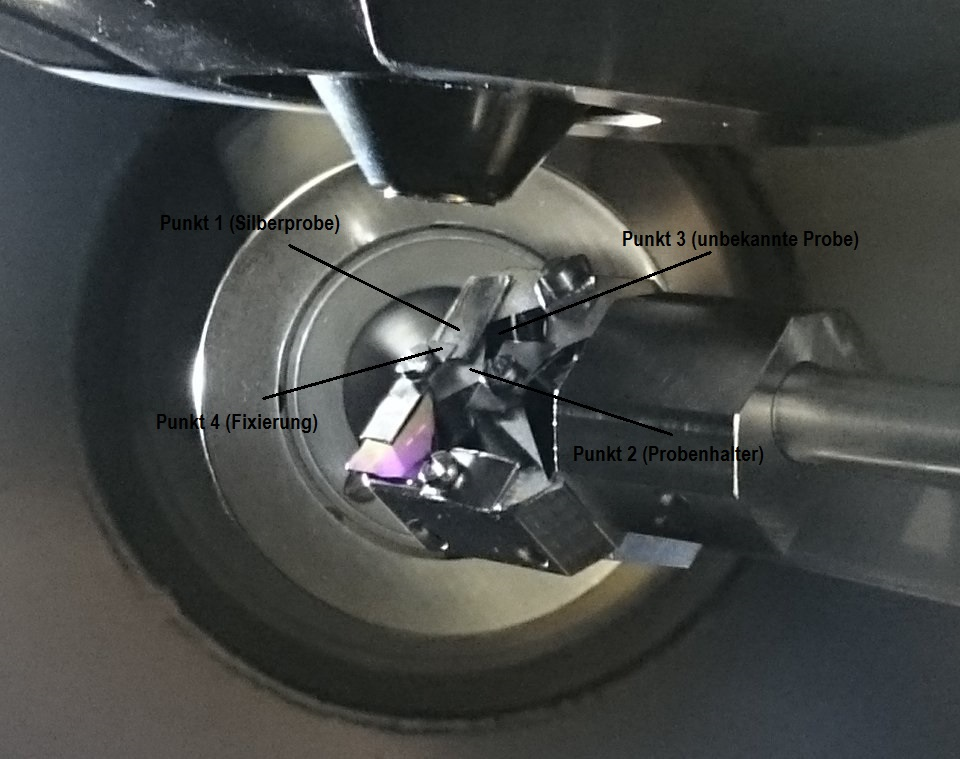
\includegraphics[scale=0.4]{probe_photo_Bear.jpg}
		\caption{\centering Bild des Probenhalters mit den untersuchten Proben \\ (Aufnahme durch eine Digitalkamera)}
	\end{figure}

	Dabei entstanden folgende Probenstrombilder:

	\begin{figure}[H]
		\center
		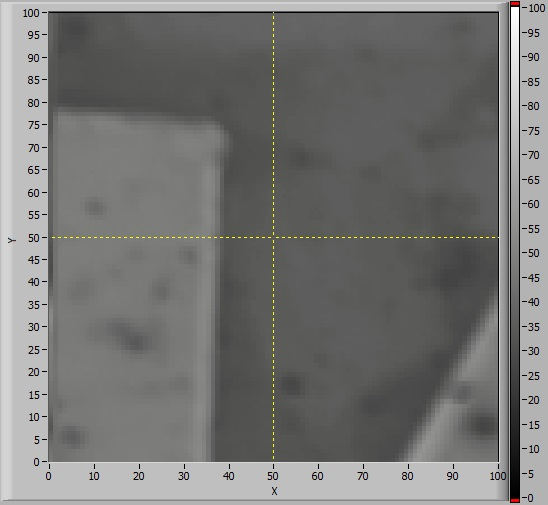
\includegraphics[scale=0.5]{epic01.jpg}
		\caption{\centering Probenstrombild von Silber (links) Probenhalter (Mitte) und Probe 3 (rechts) \\ Aufnahme mit 4keV und Probenstrom von ca. 43 nA}
	\end{figure}

	\begin{figure}[H]	
		\center
		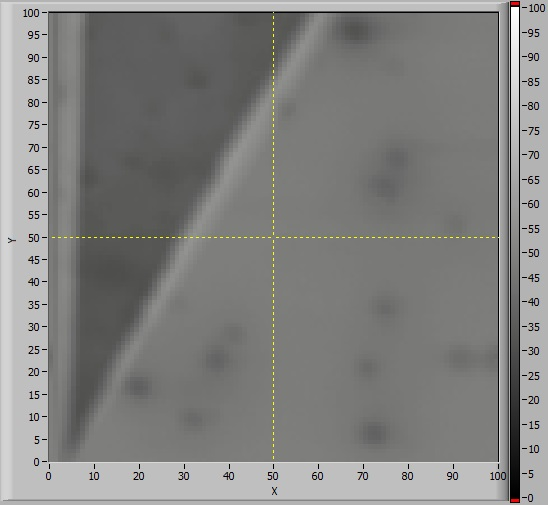
\includegraphics[scale=0.6]{epic02.jpg}
		\caption{\centering Probenstrombild von Probe 3 \\ Aufnahme mit 4keV und Probenstrom von ca. 130 nA}
	\end{figure}

	\begin{figure}[H]	
		\center
		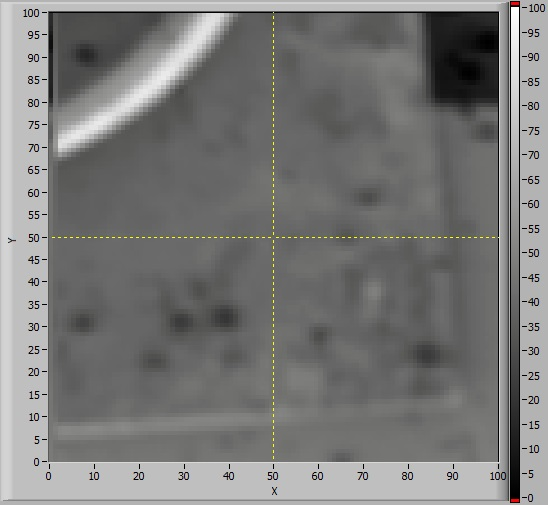
\includegraphics[scale=0.6]{epicSchraube.jpg}
		\caption{\centering Probenstrombild von Fixierung \\ Aufnahme mit 4keV und Probenstrom von ca. 110 nA}
	\end{figure}

	Die Aufnahmen stellen die jeweiligen Objekte immer horizontal gespiegelt dar. Der unterschiedliche Probenstrom deutet darauf hin, 
	dass je nach Untergrund die Elektronen mehr oder weniger stark gestreut wurden und nicht über Probe und Zählwerk zurück geleitet.

% subsection probenstrombilder (end)

\subsection{Silber-Spektrum, Messparameter und Geometriefaktor} % (fold)
\label{sub:silber_spektrum}

	\begin{figure}[H]
		\center
		% GNUPLOT: LaTeX picture with Postscript
\begingroup
  \makeatletter
  \providecommand\color[2][]{%
    \GenericError{(gnuplot) \space\space\space\@spaces}{%
      Package color not loaded in conjunction with
      terminal option `colourtext'%
    }{See the gnuplot documentation for explanation.%
    }{Either use 'blacktext' in gnuplot or load the package
      color.sty in LaTeX.}%
    \renewcommand\color[2][]{}%
  }%
  \providecommand\includegraphics[2][]{%
    \GenericError{(gnuplot) \space\space\space\@spaces}{%
      Package graphicx or graphics not loaded%
    }{See the gnuplot documentation for explanation.%
    }{The gnuplot epslatex terminal needs graphicx.sty or graphics.sty.}%
    \renewcommand\includegraphics[2][]{}%
  }%
  \providecommand\rotatebox[2]{#2}%
  \@ifundefined{ifGPcolor}{%
    \newif\ifGPcolor
    \GPcolorfalse
  }{}%
  \@ifundefined{ifGPblacktext}{%
    \newif\ifGPblacktext
    \GPblacktexttrue
  }{}%
  % define a \g@addto@macro without @ in the name:
  \let\gplgaddtomacro\g@addto@macro
  % define empty templates for all commands taking text:
  \gdef\gplbacktext{}%
  \gdef\gplfronttext{}%
  \makeatother
  \ifGPblacktext
    % no textcolor at all
    \def\colorrgb#1{}%
    \def\colorgray#1{}%
  \else
    % gray or color?
    \ifGPcolor
      \def\colorrgb#1{\color[rgb]{#1}}%
      \def\colorgray#1{\color[gray]{#1}}%
      \expandafter\def\csname LTw\endcsname{\color{white}}%
      \expandafter\def\csname LTb\endcsname{\color{black}}%
      \expandafter\def\csname LTa\endcsname{\color{black}}%
      \expandafter\def\csname LT0\endcsname{\color[rgb]{1,0,0}}%
      \expandafter\def\csname LT1\endcsname{\color[rgb]{0,1,0}}%
      \expandafter\def\csname LT2\endcsname{\color[rgb]{0,0,1}}%
      \expandafter\def\csname LT3\endcsname{\color[rgb]{1,0,1}}%
      \expandafter\def\csname LT4\endcsname{\color[rgb]{0,1,1}}%
      \expandafter\def\csname LT5\endcsname{\color[rgb]{1,1,0}}%
      \expandafter\def\csname LT6\endcsname{\color[rgb]{0,0,0}}%
      \expandafter\def\csname LT7\endcsname{\color[rgb]{1,0.3,0}}%
      \expandafter\def\csname LT8\endcsname{\color[rgb]{0.5,0.5,0.5}}%
    \else
      % gray
      \def\colorrgb#1{\color{black}}%
      \def\colorgray#1{\color[gray]{#1}}%
      \expandafter\def\csname LTw\endcsname{\color{white}}%
      \expandafter\def\csname LTb\endcsname{\color{black}}%
      \expandafter\def\csname LTa\endcsname{\color{black}}%
      \expandafter\def\csname LT0\endcsname{\color{black}}%
      \expandafter\def\csname LT1\endcsname{\color{black}}%
      \expandafter\def\csname LT2\endcsname{\color{black}}%
      \expandafter\def\csname LT3\endcsname{\color{black}}%
      \expandafter\def\csname LT4\endcsname{\color{black}}%
      \expandafter\def\csname LT5\endcsname{\color{black}}%
      \expandafter\def\csname LT6\endcsname{\color{black}}%
      \expandafter\def\csname LT7\endcsname{\color{black}}%
      \expandafter\def\csname LT8\endcsname{\color{black}}%
    \fi
  \fi
  \setlength{\unitlength}{0.0500bp}%
  \begin{picture}(9354.00,5102.00)%
    \gplgaddtomacro\gplbacktext{%
      \csname LTb\endcsname%
      \put(946,704){\makebox(0,0)[r]{\strut{}-2}}%
      \put(946,1171){\makebox(0,0)[r]{\strut{}-1.5}}%
      \put(946,1638){\makebox(0,0)[r]{\strut{}-1}}%
      \put(946,2105){\makebox(0,0)[r]{\strut{}-0.5}}%
      \put(946,2573){\makebox(0,0)[r]{\strut{} 0}}%
      \put(946,3040){\makebox(0,0)[r]{\strut{} 0.5}}%
      \put(946,3507){\makebox(0,0)[r]{\strut{} 1}}%
      \put(946,3974){\makebox(0,0)[r]{\strut{} 1.5}}%
      \put(946,4441){\makebox(0,0)[r]{\strut{} 2}}%
      \put(1078,484){\makebox(0,0){\strut{} 0}}%
      \put(2391,484){\makebox(0,0){\strut{} 100}}%
      \put(3704,484){\makebox(0,0){\strut{} 200}}%
      \put(5018,484){\makebox(0,0){\strut{} 300}}%
      \put(6331,484){\makebox(0,0){\strut{} 400}}%
      \put(7644,484){\makebox(0,0){\strut{} 500}}%
      \put(8957,484){\makebox(0,0){\strut{} 600}}%
      \put(176,2572){\rotatebox{-270}{\makebox(0,0){\strut{}$dN/dE \ [1]$}}}%
      \put(5017,154){\makebox(0,0){\strut{}$E \ [eV]$}}%
      \put(5017,4771){\makebox(0,0){\strut{}Ag-Spektrum}}%
    }%
    \gplgaddtomacro\gplfronttext{%
      \csname LTb\endcsname%
      \put(7970,4268){\makebox(0,0)[r]{\strut{}Messwerte}}%
    }%
    \gplbacktext
    \put(0,0){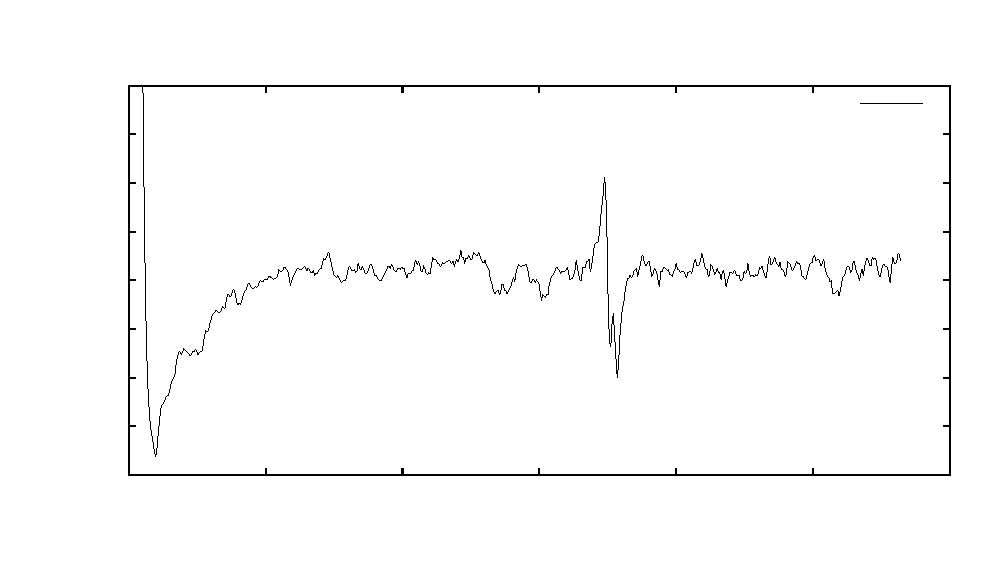
\includegraphics{ma03-16}}%
    \gplfronttext
  \end{picture}%
\endgroup

		\caption{\centering Parameter: Modulationsspannung 2V, AQ 120s, Empfindlichkeit 1mV, Zeitkonstante 300ms, Phase 12^\circ}
	\end{figure}

	\begin{figure}[H]
		\center
		% GNUPLOT: LaTeX picture with Postscript
\begingroup
  \makeatletter
  \providecommand\color[2][]{%
    \GenericError{(gnuplot) \space\space\space\@spaces}{%
      Package color not loaded in conjunction with
      terminal option `colourtext'%
    }{See the gnuplot documentation for explanation.%
    }{Either use 'blacktext' in gnuplot or load the package
      color.sty in LaTeX.}%
    \renewcommand\color[2][]{}%
  }%
  \providecommand\includegraphics[2][]{%
    \GenericError{(gnuplot) \space\space\space\@spaces}{%
      Package graphicx or graphics not loaded%
    }{See the gnuplot documentation for explanation.%
    }{The gnuplot epslatex terminal needs graphicx.sty or graphics.sty.}%
    \renewcommand\includegraphics[2][]{}%
  }%
  \providecommand\rotatebox[2]{#2}%
  \@ifundefined{ifGPcolor}{%
    \newif\ifGPcolor
    \GPcolorfalse
  }{}%
  \@ifundefined{ifGPblacktext}{%
    \newif\ifGPblacktext
    \GPblacktexttrue
  }{}%
  % define a \g@addto@macro without @ in the name:
  \let\gplgaddtomacro\g@addto@macro
  % define empty templates for all commands taking text:
  \gdef\gplbacktext{}%
  \gdef\gplfronttext{}%
  \makeatother
  \ifGPblacktext
    % no textcolor at all
    \def\colorrgb#1{}%
    \def\colorgray#1{}%
  \else
    % gray or color?
    \ifGPcolor
      \def\colorrgb#1{\color[rgb]{#1}}%
      \def\colorgray#1{\color[gray]{#1}}%
      \expandafter\def\csname LTw\endcsname{\color{white}}%
      \expandafter\def\csname LTb\endcsname{\color{black}}%
      \expandafter\def\csname LTa\endcsname{\color{black}}%
      \expandafter\def\csname LT0\endcsname{\color[rgb]{1,0,0}}%
      \expandafter\def\csname LT1\endcsname{\color[rgb]{0,1,0}}%
      \expandafter\def\csname LT2\endcsname{\color[rgb]{0,0,1}}%
      \expandafter\def\csname LT3\endcsname{\color[rgb]{1,0,1}}%
      \expandafter\def\csname LT4\endcsname{\color[rgb]{0,1,1}}%
      \expandafter\def\csname LT5\endcsname{\color[rgb]{1,1,0}}%
      \expandafter\def\csname LT6\endcsname{\color[rgb]{0,0,0}}%
      \expandafter\def\csname LT7\endcsname{\color[rgb]{1,0.3,0}}%
      \expandafter\def\csname LT8\endcsname{\color[rgb]{0.5,0.5,0.5}}%
    \else
      % gray
      \def\colorrgb#1{\color{black}}%
      \def\colorgray#1{\color[gray]{#1}}%
      \expandafter\def\csname LTw\endcsname{\color{white}}%
      \expandafter\def\csname LTb\endcsname{\color{black}}%
      \expandafter\def\csname LTa\endcsname{\color{black}}%
      \expandafter\def\csname LT0\endcsname{\color{black}}%
      \expandafter\def\csname LT1\endcsname{\color{black}}%
      \expandafter\def\csname LT2\endcsname{\color{black}}%
      \expandafter\def\csname LT3\endcsname{\color{black}}%
      \expandafter\def\csname LT4\endcsname{\color{black}}%
      \expandafter\def\csname LT5\endcsname{\color{black}}%
      \expandafter\def\csname LT6\endcsname{\color{black}}%
      \expandafter\def\csname LT7\endcsname{\color{black}}%
      \expandafter\def\csname LT8\endcsname{\color{black}}%
    \fi
  \fi
  \setlength{\unitlength}{0.0500bp}%
  \begin{picture}(9354.00,5102.00)%
    \gplgaddtomacro\gplbacktext{%
      \csname LTb\endcsname%
      \put(946,704){\makebox(0,0)[r]{\strut{}-2}}%
      \put(946,1238){\makebox(0,0)[r]{\strut{}-1.5}}%
      \put(946,1772){\makebox(0,0)[r]{\strut{}-1}}%
      \put(946,2306){\makebox(0,0)[r]{\strut{}-0.5}}%
      \put(946,2839){\makebox(0,0)[r]{\strut{} 0}}%
      \put(946,3373){\makebox(0,0)[r]{\strut{} 0.5}}%
      \put(946,3907){\makebox(0,0)[r]{\strut{} 1}}%
      \put(946,4441){\makebox(0,0)[r]{\strut{} 1.5}}%
      \put(1078,484){\makebox(0,0){\strut{} 310}}%
      \put(1953,484){\makebox(0,0){\strut{} 320}}%
      \put(2829,484){\makebox(0,0){\strut{} 330}}%
      \put(3704,484){\makebox(0,0){\strut{} 340}}%
      \put(4580,484){\makebox(0,0){\strut{} 350}}%
      \put(5455,484){\makebox(0,0){\strut{} 360}}%
      \put(6331,484){\makebox(0,0){\strut{} 370}}%
      \put(7206,484){\makebox(0,0){\strut{} 380}}%
      \put(8082,484){\makebox(0,0){\strut{} 390}}%
      \put(8957,484){\makebox(0,0){\strut{} 400}}%
      \put(176,2572){\rotatebox{-270}{\makebox(0,0){\strut{}$dN/dE \ [1]$}}}%
      \put(5017,154){\makebox(0,0){\strut{}$E \ [eV]$}}%
      \put(5017,4771){\makebox(0,0){\strut{}Ag-Spektrum}}%
    }%
    \gplgaddtomacro\gplfronttext{%
      \csname LTb\endcsname%
      \put(7970,4268){\makebox(0,0)[r]{\strut{}Messwerte}}%
    }%
    \gplbacktext
    \put(0,0){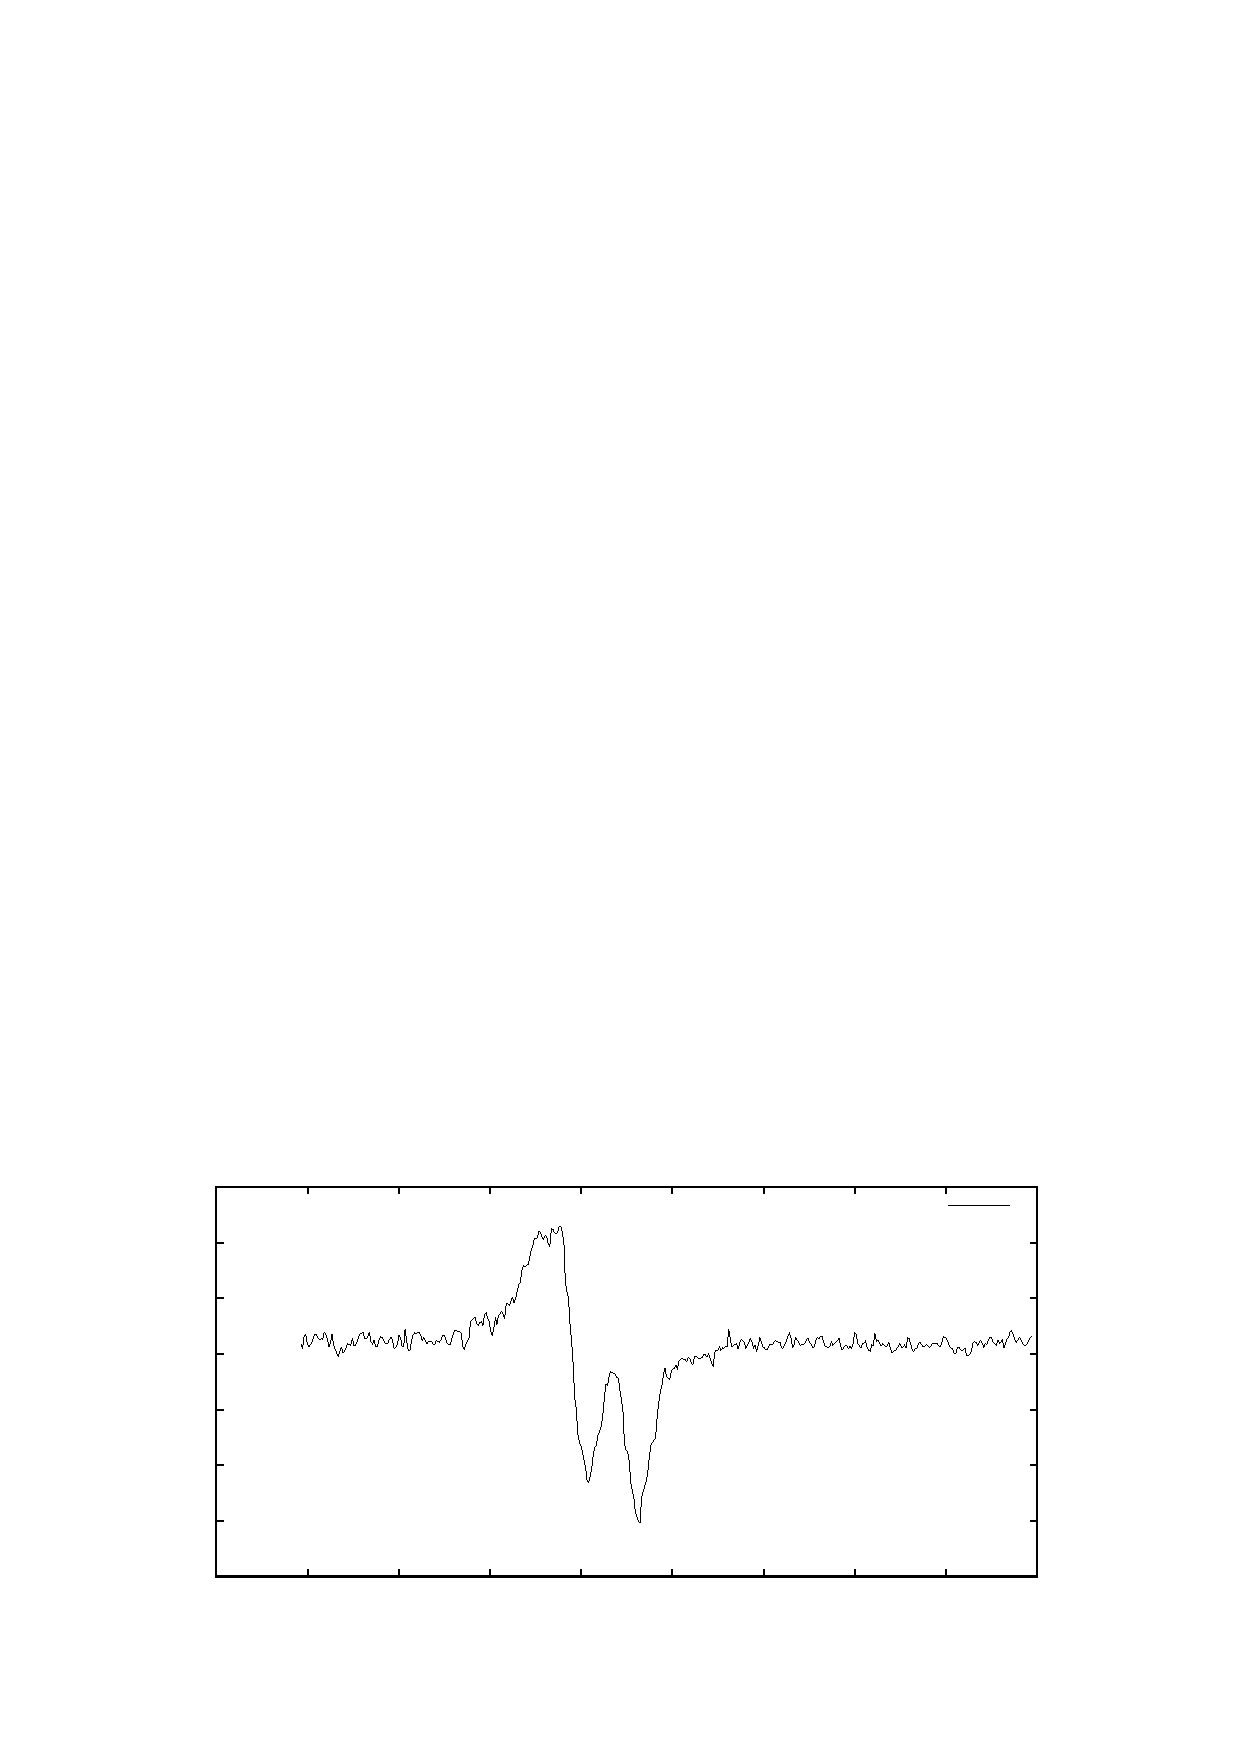
\includegraphics{ma03-15}}%
    \gplfronttext
  \end{picture}%
\endgroup

		\caption{\centering Parameter: Modulationsspannung 2V, AQ 120s, Empfindlichkeit 1mV, Zeitkonstante 300ms, Phase 12^\circ}
	\end{figure}

	Zu sehen ist das Auger-Elektronen-Spektrum von Silber (Ag) in differentieller Form in einem CMA-Spannungsbereich von 0 bis 350 V.
	Und damit in einem Energiebereich von 0 bis 570 eV (Geometriefaktor K = 1,624 siehe unten).
	Gut zu erkennen ist der charakteristische Doppelpeak. 
	Die beiden Minima sind im vergrößertem Ausschnitt abzulesen:

	Dabei konnten im verwendeten Messprogramm folgende Werte abgelesen werden:
	\begin{itemize}
		\item
			$U_{min}^{(1)} = 216.0V$ 
		\item
			$U_{min}^{(2)} = 219.4V$
	\end{itemize}

	Der Geometriefaktor K wurde anhand dieser beiden Peaks und den zugehörigen Tabellenwerten 351eV bzw. 356eV bestimmt (dem Katalog am Versuchsplatz entnommen):
	\begin{itemize}
		\item
			$K_1 = \dfrac{351}{216.0} = 1.625$
		\item
			$K_2 = \dfrac{356}{219.4} = 1.623$
	\end{itemize}
	\[
		\Rightarrow \={K} = 1.624
	\]
	Alle weiteren Auger-Spektren wurden mit diesem Geometriefaktor skaliert.
	Im Folgenden soll nun der Einfluss der verschiedenen Messparameter betrachtet werden.

	\subsubsection{Modulationsspannung} % (fold)
	\label{ssub:modulationsspannung}
	
		\begin{figure}[H]
			\center
			% GNUPLOT: LaTeX picture with Postscript
\begingroup
  \makeatletter
  \providecommand\color[2][]{%
    \GenericError{(gnuplot) \space\space\space\@spaces}{%
      Package color not loaded in conjunction with
      terminal option `colourtext'%
    }{See the gnuplot documentation for explanation.%
    }{Either use 'blacktext' in gnuplot or load the package
      color.sty in LaTeX.}%
    \renewcommand\color[2][]{}%
  }%
  \providecommand\includegraphics[2][]{%
    \GenericError{(gnuplot) \space\space\space\@spaces}{%
      Package graphicx or graphics not loaded%
    }{See the gnuplot documentation for explanation.%
    }{The gnuplot epslatex terminal needs graphicx.sty or graphics.sty.}%
    \renewcommand\includegraphics[2][]{}%
  }%
  \providecommand\rotatebox[2]{#2}%
  \@ifundefined{ifGPcolor}{%
    \newif\ifGPcolor
    \GPcolorfalse
  }{}%
  \@ifundefined{ifGPblacktext}{%
    \newif\ifGPblacktext
    \GPblacktexttrue
  }{}%
  % define a \g@addto@macro without @ in the name:
  \let\gplgaddtomacro\g@addto@macro
  % define empty templates for all commands taking text:
  \gdef\gplbacktext{}%
  \gdef\gplfronttext{}%
  \makeatother
  \ifGPblacktext
    % no textcolor at all
    \def\colorrgb#1{}%
    \def\colorgray#1{}%
  \else
    % gray or color?
    \ifGPcolor
      \def\colorrgb#1{\color[rgb]{#1}}%
      \def\colorgray#1{\color[gray]{#1}}%
      \expandafter\def\csname LTw\endcsname{\color{white}}%
      \expandafter\def\csname LTb\endcsname{\color{black}}%
      \expandafter\def\csname LTa\endcsname{\color{black}}%
      \expandafter\def\csname LT0\endcsname{\color[rgb]{1,0,0}}%
      \expandafter\def\csname LT1\endcsname{\color[rgb]{0,1,0}}%
      \expandafter\def\csname LT2\endcsname{\color[rgb]{0,0,1}}%
      \expandafter\def\csname LT3\endcsname{\color[rgb]{1,0,1}}%
      \expandafter\def\csname LT4\endcsname{\color[rgb]{0,1,1}}%
      \expandafter\def\csname LT5\endcsname{\color[rgb]{1,1,0}}%
      \expandafter\def\csname LT6\endcsname{\color[rgb]{0,0,0}}%
      \expandafter\def\csname LT7\endcsname{\color[rgb]{1,0.3,0}}%
      \expandafter\def\csname LT8\endcsname{\color[rgb]{0.5,0.5,0.5}}%
    \else
      % gray
      \def\colorrgb#1{\color{black}}%
      \def\colorgray#1{\color[gray]{#1}}%
      \expandafter\def\csname LTw\endcsname{\color{white}}%
      \expandafter\def\csname LTb\endcsname{\color{black}}%
      \expandafter\def\csname LTa\endcsname{\color{black}}%
      \expandafter\def\csname LT0\endcsname{\color{black}}%
      \expandafter\def\csname LT1\endcsname{\color{black}}%
      \expandafter\def\csname LT2\endcsname{\color{black}}%
      \expandafter\def\csname LT3\endcsname{\color{black}}%
      \expandafter\def\csname LT4\endcsname{\color{black}}%
      \expandafter\def\csname LT5\endcsname{\color{black}}%
      \expandafter\def\csname LT6\endcsname{\color{black}}%
      \expandafter\def\csname LT7\endcsname{\color{black}}%
      \expandafter\def\csname LT8\endcsname{\color{black}}%
    \fi
  \fi
  \setlength{\unitlength}{0.0500bp}%
  \begin{picture}(9354.00,5102.00)%
    \gplgaddtomacro\gplbacktext{%
      \csname LTb\endcsname%
      \put(682,704){\makebox(0,0)[r]{\strut{}-4}}%
      \put(682,1171){\makebox(0,0)[r]{\strut{}-3}}%
      \put(682,1638){\makebox(0,0)[r]{\strut{}-2}}%
      \put(682,2105){\makebox(0,0)[r]{\strut{}-1}}%
      \put(682,2573){\makebox(0,0)[r]{\strut{} 0}}%
      \put(682,3040){\makebox(0,0)[r]{\strut{} 1}}%
      \put(682,3507){\makebox(0,0)[r]{\strut{} 2}}%
      \put(682,3974){\makebox(0,0)[r]{\strut{} 3}}%
      \put(682,4441){\makebox(0,0)[r]{\strut{} 4}}%
      \put(814,484){\makebox(0,0){\strut{} 0}}%
      \put(2171,484){\makebox(0,0){\strut{} 100}}%
      \put(3528,484){\makebox(0,0){\strut{} 200}}%
      \put(4886,484){\makebox(0,0){\strut{} 300}}%
      \put(6243,484){\makebox(0,0){\strut{} 400}}%
      \put(7600,484){\makebox(0,0){\strut{} 500}}%
      \put(8957,484){\makebox(0,0){\strut{} 600}}%
      \put(176,2572){\rotatebox{-270}{\makebox(0,0){\strut{}$dN/dE \ [1]$}}}%
      \put(4885,154){\makebox(0,0){\strut{}$E \ [eV]$}}%
      \put(4885,4771){\makebox(0,0){\strut{}Ag-Spektrum mit Modulationsspannung $2V$}}%
    }%
    \gplgaddtomacro\gplfronttext{%
      \csname LTb\endcsname%
      \put(7970,4268){\makebox(0,0)[r]{\strut{}Messwerte}}%
    }%
    \gplbacktext
    \put(0,0){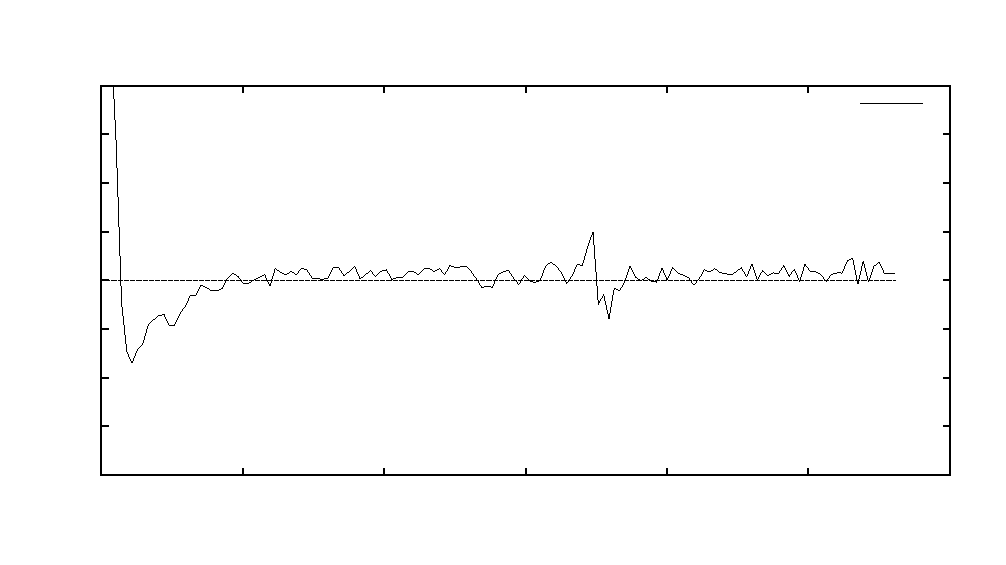
\includegraphics{ma03-01}}%
    \gplfronttext
  \end{picture}%
\endgroup

			\caption{\centering Parameter: AQ 30s, Empfindlichkeit 1mV, Zeitkonstante 100ms, Phase 0^\circ}
		\end{figure}

		\begin{figure}[H]
			\center
			% GNUPLOT: LaTeX picture with Postscript
\begingroup
  \makeatletter
  \providecommand\color[2][]{%
    \GenericError{(gnuplot) \space\space\space\@spaces}{%
      Package color not loaded in conjunction with
      terminal option `colourtext'%
    }{See the gnuplot documentation for explanation.%
    }{Either use 'blacktext' in gnuplot or load the package
      color.sty in LaTeX.}%
    \renewcommand\color[2][]{}%
  }%
  \providecommand\includegraphics[2][]{%
    \GenericError{(gnuplot) \space\space\space\@spaces}{%
      Package graphicx or graphics not loaded%
    }{See the gnuplot documentation for explanation.%
    }{The gnuplot epslatex terminal needs graphicx.sty or graphics.sty.}%
    \renewcommand\includegraphics[2][]{}%
  }%
  \providecommand\rotatebox[2]{#2}%
  \@ifundefined{ifGPcolor}{%
    \newif\ifGPcolor
    \GPcolorfalse
  }{}%
  \@ifundefined{ifGPblacktext}{%
    \newif\ifGPblacktext
    \GPblacktexttrue
  }{}%
  % define a \g@addto@macro without @ in the name:
  \let\gplgaddtomacro\g@addto@macro
  % define empty templates for all commands taking text:
  \gdef\gplbacktext{}%
  \gdef\gplfronttext{}%
  \makeatother
  \ifGPblacktext
    % no textcolor at all
    \def\colorrgb#1{}%
    \def\colorgray#1{}%
  \else
    % gray or color?
    \ifGPcolor
      \def\colorrgb#1{\color[rgb]{#1}}%
      \def\colorgray#1{\color[gray]{#1}}%
      \expandafter\def\csname LTw\endcsname{\color{white}}%
      \expandafter\def\csname LTb\endcsname{\color{black}}%
      \expandafter\def\csname LTa\endcsname{\color{black}}%
      \expandafter\def\csname LT0\endcsname{\color[rgb]{1,0,0}}%
      \expandafter\def\csname LT1\endcsname{\color[rgb]{0,1,0}}%
      \expandafter\def\csname LT2\endcsname{\color[rgb]{0,0,1}}%
      \expandafter\def\csname LT3\endcsname{\color[rgb]{1,0,1}}%
      \expandafter\def\csname LT4\endcsname{\color[rgb]{0,1,1}}%
      \expandafter\def\csname LT5\endcsname{\color[rgb]{1,1,0}}%
      \expandafter\def\csname LT6\endcsname{\color[rgb]{0,0,0}}%
      \expandafter\def\csname LT7\endcsname{\color[rgb]{1,0.3,0}}%
      \expandafter\def\csname LT8\endcsname{\color[rgb]{0.5,0.5,0.5}}%
    \else
      % gray
      \def\colorrgb#1{\color{black}}%
      \def\colorgray#1{\color[gray]{#1}}%
      \expandafter\def\csname LTw\endcsname{\color{white}}%
      \expandafter\def\csname LTb\endcsname{\color{black}}%
      \expandafter\def\csname LTa\endcsname{\color{black}}%
      \expandafter\def\csname LT0\endcsname{\color{black}}%
      \expandafter\def\csname LT1\endcsname{\color{black}}%
      \expandafter\def\csname LT2\endcsname{\color{black}}%
      \expandafter\def\csname LT3\endcsname{\color{black}}%
      \expandafter\def\csname LT4\endcsname{\color{black}}%
      \expandafter\def\csname LT5\endcsname{\color{black}}%
      \expandafter\def\csname LT6\endcsname{\color{black}}%
      \expandafter\def\csname LT7\endcsname{\color{black}}%
      \expandafter\def\csname LT8\endcsname{\color{black}}%
    \fi
  \fi
  \setlength{\unitlength}{0.0500bp}%
  \begin{picture}(9354.00,5102.00)%
    \gplgaddtomacro\gplbacktext{%
      \csname LTb\endcsname%
      \put(682,704){\makebox(0,0)[r]{\strut{}-4}}%
      \put(682,1171){\makebox(0,0)[r]{\strut{}-3}}%
      \put(682,1638){\makebox(0,0)[r]{\strut{}-2}}%
      \put(682,2105){\makebox(0,0)[r]{\strut{}-1}}%
      \put(682,2573){\makebox(0,0)[r]{\strut{} 0}}%
      \put(682,3040){\makebox(0,0)[r]{\strut{} 1}}%
      \put(682,3507){\makebox(0,0)[r]{\strut{} 2}}%
      \put(682,3974){\makebox(0,0)[r]{\strut{} 3}}%
      \put(682,4441){\makebox(0,0)[r]{\strut{} 4}}%
      \put(814,484){\makebox(0,0){\strut{} 0}}%
      \put(2171,484){\makebox(0,0){\strut{} 100}}%
      \put(3528,484){\makebox(0,0){\strut{} 200}}%
      \put(4886,484){\makebox(0,0){\strut{} 300}}%
      \put(6243,484){\makebox(0,0){\strut{} 400}}%
      \put(7600,484){\makebox(0,0){\strut{} 500}}%
      \put(8957,484){\makebox(0,0){\strut{} 600}}%
      \put(176,2572){\rotatebox{-270}{\makebox(0,0){\strut{}$dN/dE \ [1]$}}}%
      \put(4885,154){\makebox(0,0){\strut{}$E \ [eV]$}}%
      \put(4885,4771){\makebox(0,0){\strut{}Ag-Spektrum mit Modulationsspannung $5V$}}%
    }%
    \gplgaddtomacro\gplfronttext{%
      \csname LTb\endcsname%
      \put(7970,4268){\makebox(0,0)[r]{\strut{}Messwerte}}%
    }%
    \gplbacktext
    \put(0,0){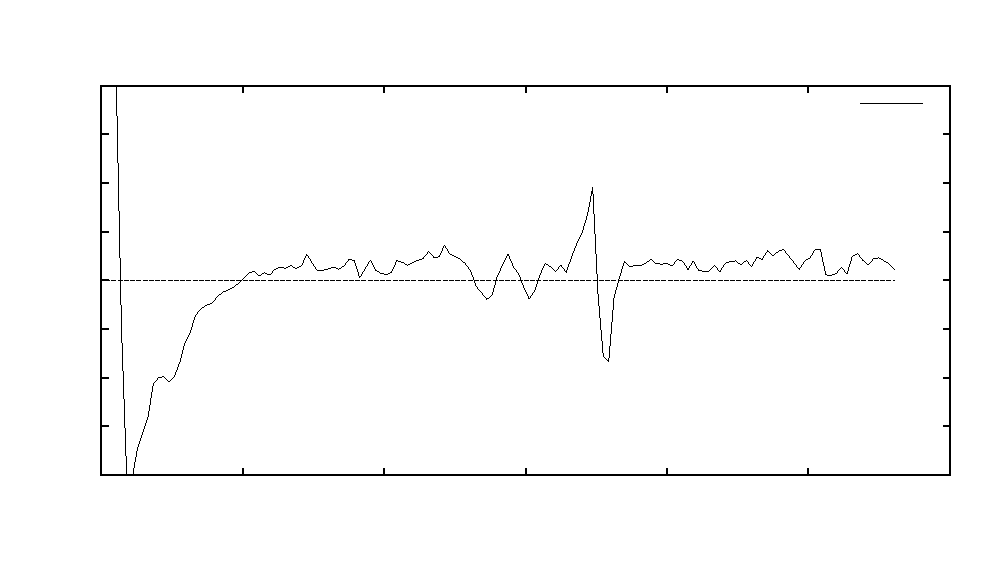
\includegraphics{ma03-02}}%
    \gplfronttext
  \end{picture}%
\endgroup

			\caption{\centering Parameter: AQ 30s, Empfindlichkeit 1mV, Zeitkonstante 100ms, Phase 0^\circ}	
		\end{figure}

		\begin{figure}[H]
			\center
			% GNUPLOT: LaTeX picture with Postscript
\begingroup
  \makeatletter
  \providecommand\color[2][]{%
    \GenericError{(gnuplot) \space\space\space\@spaces}{%
      Package color not loaded in conjunction with
      terminal option `colourtext'%
    }{See the gnuplot documentation for explanation.%
    }{Either use 'blacktext' in gnuplot or load the package
      color.sty in LaTeX.}%
    \renewcommand\color[2][]{}%
  }%
  \providecommand\includegraphics[2][]{%
    \GenericError{(gnuplot) \space\space\space\@spaces}{%
      Package graphicx or graphics not loaded%
    }{See the gnuplot documentation for explanation.%
    }{The gnuplot epslatex terminal needs graphicx.sty or graphics.sty.}%
    \renewcommand\includegraphics[2][]{}%
  }%
  \providecommand\rotatebox[2]{#2}%
  \@ifundefined{ifGPcolor}{%
    \newif\ifGPcolor
    \GPcolorfalse
  }{}%
  \@ifundefined{ifGPblacktext}{%
    \newif\ifGPblacktext
    \GPblacktexttrue
  }{}%
  % define a \g@addto@macro without @ in the name:
  \let\gplgaddtomacro\g@addto@macro
  % define empty templates for all commands taking text:
  \gdef\gplbacktext{}%
  \gdef\gplfronttext{}%
  \makeatother
  \ifGPblacktext
    % no textcolor at all
    \def\colorrgb#1{}%
    \def\colorgray#1{}%
  \else
    % gray or color?
    \ifGPcolor
      \def\colorrgb#1{\color[rgb]{#1}}%
      \def\colorgray#1{\color[gray]{#1}}%
      \expandafter\def\csname LTw\endcsname{\color{white}}%
      \expandafter\def\csname LTb\endcsname{\color{black}}%
      \expandafter\def\csname LTa\endcsname{\color{black}}%
      \expandafter\def\csname LT0\endcsname{\color[rgb]{1,0,0}}%
      \expandafter\def\csname LT1\endcsname{\color[rgb]{0,1,0}}%
      \expandafter\def\csname LT2\endcsname{\color[rgb]{0,0,1}}%
      \expandafter\def\csname LT3\endcsname{\color[rgb]{1,0,1}}%
      \expandafter\def\csname LT4\endcsname{\color[rgb]{0,1,1}}%
      \expandafter\def\csname LT5\endcsname{\color[rgb]{1,1,0}}%
      \expandafter\def\csname LT6\endcsname{\color[rgb]{0,0,0}}%
      \expandafter\def\csname LT7\endcsname{\color[rgb]{1,0.3,0}}%
      \expandafter\def\csname LT8\endcsname{\color[rgb]{0.5,0.5,0.5}}%
    \else
      % gray
      \def\colorrgb#1{\color{black}}%
      \def\colorgray#1{\color[gray]{#1}}%
      \expandafter\def\csname LTw\endcsname{\color{white}}%
      \expandafter\def\csname LTb\endcsname{\color{black}}%
      \expandafter\def\csname LTa\endcsname{\color{black}}%
      \expandafter\def\csname LT0\endcsname{\color{black}}%
      \expandafter\def\csname LT1\endcsname{\color{black}}%
      \expandafter\def\csname LT2\endcsname{\color{black}}%
      \expandafter\def\csname LT3\endcsname{\color{black}}%
      \expandafter\def\csname LT4\endcsname{\color{black}}%
      \expandafter\def\csname LT5\endcsname{\color{black}}%
      \expandafter\def\csname LT6\endcsname{\color{black}}%
      \expandafter\def\csname LT7\endcsname{\color{black}}%
      \expandafter\def\csname LT8\endcsname{\color{black}}%
    \fi
  \fi
  \setlength{\unitlength}{0.0500bp}%
  \begin{picture}(9354.00,5102.00)%
    \gplgaddtomacro\gplbacktext{%
      \csname LTb\endcsname%
      \put(682,704){\makebox(0,0)[r]{\strut{}-4}}%
      \put(682,1171){\makebox(0,0)[r]{\strut{}-3}}%
      \put(682,1638){\makebox(0,0)[r]{\strut{}-2}}%
      \put(682,2105){\makebox(0,0)[r]{\strut{}-1}}%
      \put(682,2573){\makebox(0,0)[r]{\strut{} 0}}%
      \put(682,3040){\makebox(0,0)[r]{\strut{} 1}}%
      \put(682,3507){\makebox(0,0)[r]{\strut{} 2}}%
      \put(682,3974){\makebox(0,0)[r]{\strut{} 3}}%
      \put(682,4441){\makebox(0,0)[r]{\strut{} 4}}%
      \put(814,484){\makebox(0,0){\strut{} 0}}%
      \put(2171,484){\makebox(0,0){\strut{} 100}}%
      \put(3528,484){\makebox(0,0){\strut{} 200}}%
      \put(4886,484){\makebox(0,0){\strut{} 300}}%
      \put(6243,484){\makebox(0,0){\strut{} 400}}%
      \put(7600,484){\makebox(0,0){\strut{} 500}}%
      \put(8957,484){\makebox(0,0){\strut{} 600}}%
      \put(176,2572){\rotatebox{-270}{\makebox(0,0){\strut{}$dN/dE \ [1]$}}}%
      \put(4885,154){\makebox(0,0){\strut{}$E \ [eV]$}}%
      \put(4885,4771){\makebox(0,0){\strut{}Ag-Spektrummit Modulationsspannung 10V}}%
    }%
    \gplgaddtomacro\gplfronttext{%
      \csname LTb\endcsname%
      \put(7970,4268){\makebox(0,0)[r]{\strut{}Messwerte}}%
    }%
    \gplbacktext
    \put(0,0){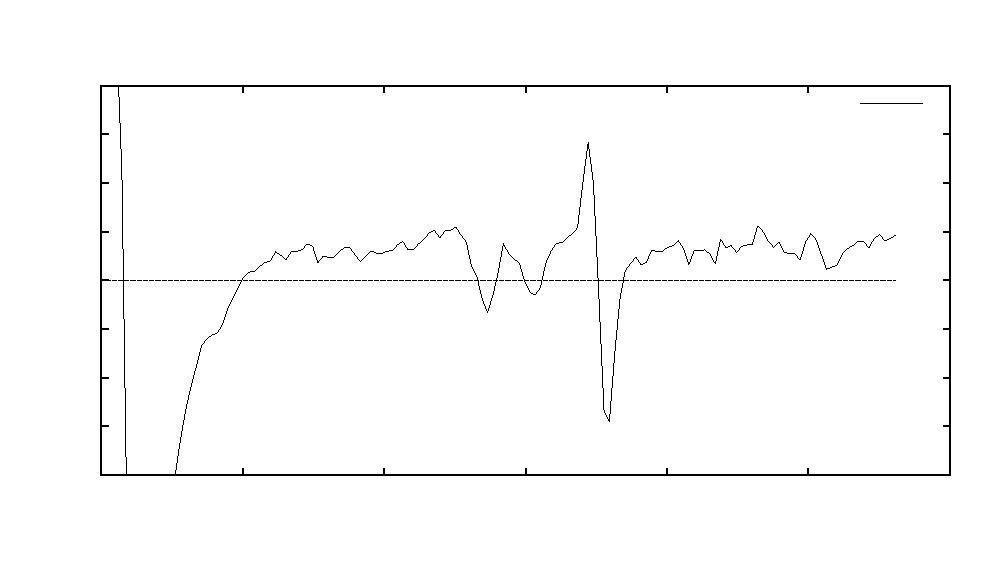
\includegraphics{ma03-03}}%
    \gplfronttext
  \end{picture}%
\endgroup

			\caption{\centering Parameter: AQ 30s, Empfindlichkeit 1mV, Zeitkonstante 100ms, Phase 0^\circ}
		\end{figure}
	
		Betrachtet man Peak-Höhe und Rauschen so fällt auf, dass die Silberpeaks bei 5V doppelt so hoch sind (bei gleicher Empfindlichkeit, Skalierung etc.), wie bei 2V.
		Dagegen hat das Rauschen nur minimal bis nicht zugenommen hat. 
		Allerdings zeigt sich auf vielen Bildern mit 10V Modulation, dass das Rauschen zwar nicht unbedingt an Intensität zunimmt, aber die Kurven im Allgemeinen nach oben verschoben ist. 
		Auf jeden Fall lässt sich durch höhere Modulationsspannung ein besseres Signal/Rausch-Verhältnis erhalten.
		Damit verstärken sich die Extrema, wobei jedoch zu beachten ist, dass keine Peak Abstände unterhalb der Modulationsspannung mehr aufgelöst werden können, da über diese hinweg gemittelt wird. 
		Die Kurve wird also glatter.

	% subsubsection modulationsspannung (end)

	\subsubsection{Zeitkonstante} % (fold)
	\label{ssub:zeitkonstante}
	
		Die Zeitkonstante stellt ein Maß dafür da, über wie viele Samples das Signal gemittelt wird.
		Die folgenden Spektren veranschaulichen dieses Verhalten:

		\begin{figure}[H]
			\center
			% GNUPLOT: LaTeX picture with Postscript
\begingroup
  \makeatletter
  \providecommand\color[2][]{%
    \GenericError{(gnuplot) \space\space\space\@spaces}{%
      Package color not loaded in conjunction with
      terminal option `colourtext'%
    }{See the gnuplot documentation for explanation.%
    }{Either use 'blacktext' in gnuplot or load the package
      color.sty in LaTeX.}%
    \renewcommand\color[2][]{}%
  }%
  \providecommand\includegraphics[2][]{%
    \GenericError{(gnuplot) \space\space\space\@spaces}{%
      Package graphicx or graphics not loaded%
    }{See the gnuplot documentation for explanation.%
    }{The gnuplot epslatex terminal needs graphicx.sty or graphics.sty.}%
    \renewcommand\includegraphics[2][]{}%
  }%
  \providecommand\rotatebox[2]{#2}%
  \@ifundefined{ifGPcolor}{%
    \newif\ifGPcolor
    \GPcolorfalse
  }{}%
  \@ifundefined{ifGPblacktext}{%
    \newif\ifGPblacktext
    \GPblacktexttrue
  }{}%
  % define a \g@addto@macro without @ in the name:
  \let\gplgaddtomacro\g@addto@macro
  % define empty templates for all commands taking text:
  \gdef\gplbacktext{}%
  \gdef\gplfronttext{}%
  \makeatother
  \ifGPblacktext
    % no textcolor at all
    \def\colorrgb#1{}%
    \def\colorgray#1{}%
  \else
    % gray or color?
    \ifGPcolor
      \def\colorrgb#1{\color[rgb]{#1}}%
      \def\colorgray#1{\color[gray]{#1}}%
      \expandafter\def\csname LTw\endcsname{\color{white}}%
      \expandafter\def\csname LTb\endcsname{\color{black}}%
      \expandafter\def\csname LTa\endcsname{\color{black}}%
      \expandafter\def\csname LT0\endcsname{\color[rgb]{1,0,0}}%
      \expandafter\def\csname LT1\endcsname{\color[rgb]{0,1,0}}%
      \expandafter\def\csname LT2\endcsname{\color[rgb]{0,0,1}}%
      \expandafter\def\csname LT3\endcsname{\color[rgb]{1,0,1}}%
      \expandafter\def\csname LT4\endcsname{\color[rgb]{0,1,1}}%
      \expandafter\def\csname LT5\endcsname{\color[rgb]{1,1,0}}%
      \expandafter\def\csname LT6\endcsname{\color[rgb]{0,0,0}}%
      \expandafter\def\csname LT7\endcsname{\color[rgb]{1,0.3,0}}%
      \expandafter\def\csname LT8\endcsname{\color[rgb]{0.5,0.5,0.5}}%
    \else
      % gray
      \def\colorrgb#1{\color{black}}%
      \def\colorgray#1{\color[gray]{#1}}%
      \expandafter\def\csname LTw\endcsname{\color{white}}%
      \expandafter\def\csname LTb\endcsname{\color{black}}%
      \expandafter\def\csname LTa\endcsname{\color{black}}%
      \expandafter\def\csname LT0\endcsname{\color{black}}%
      \expandafter\def\csname LT1\endcsname{\color{black}}%
      \expandafter\def\csname LT2\endcsname{\color{black}}%
      \expandafter\def\csname LT3\endcsname{\color{black}}%
      \expandafter\def\csname LT4\endcsname{\color{black}}%
      \expandafter\def\csname LT5\endcsname{\color{black}}%
      \expandafter\def\csname LT6\endcsname{\color{black}}%
      \expandafter\def\csname LT7\endcsname{\color{black}}%
      \expandafter\def\csname LT8\endcsname{\color{black}}%
    \fi
  \fi
  \setlength{\unitlength}{0.0500bp}%
  \begin{picture}(9354.00,5102.00)%
    \gplgaddtomacro\gplbacktext{%
      \csname LTb\endcsname%
      \put(682,704){\makebox(0,0)[r]{\strut{}-3}}%
      \put(682,1327){\makebox(0,0)[r]{\strut{}-2}}%
      \put(682,1950){\makebox(0,0)[r]{\strut{}-1}}%
      \put(682,2573){\makebox(0,0)[r]{\strut{} 0}}%
      \put(682,3195){\makebox(0,0)[r]{\strut{} 1}}%
      \put(682,3818){\makebox(0,0)[r]{\strut{} 2}}%
      \put(682,4441){\makebox(0,0)[r]{\strut{} 3}}%
      \put(1061,484){\makebox(0,0){\strut{} 280}}%
      \put(2048,484){\makebox(0,0){\strut{} 300}}%
      \put(3035,484){\makebox(0,0){\strut{} 320}}%
      \put(4022,484){\makebox(0,0){\strut{} 340}}%
      \put(5009,484){\makebox(0,0){\strut{} 360}}%
      \put(5996,484){\makebox(0,0){\strut{} 380}}%
      \put(6983,484){\makebox(0,0){\strut{} 400}}%
      \put(7970,484){\makebox(0,0){\strut{} 420}}%
      \put(8957,484){\makebox(0,0){\strut{} 440}}%
      \put(176,2572){\rotatebox{-270}{\makebox(0,0){\strut{}$dN/dE \ [1]$}}}%
      \put(4885,154){\makebox(0,0){\strut{}$E \ [eV]$}}%
      \put(4885,4771){\makebox(0,0){\strut{}Ag-Spektrum mit Zeitkonstante $10ms$}}%
    }%
    \gplgaddtomacro\gplfronttext{%
      \csname LTb\endcsname%
      \put(7970,4268){\makebox(0,0)[r]{\strut{}Messwerte}}%
    }%
    \gplbacktext
    \put(0,0){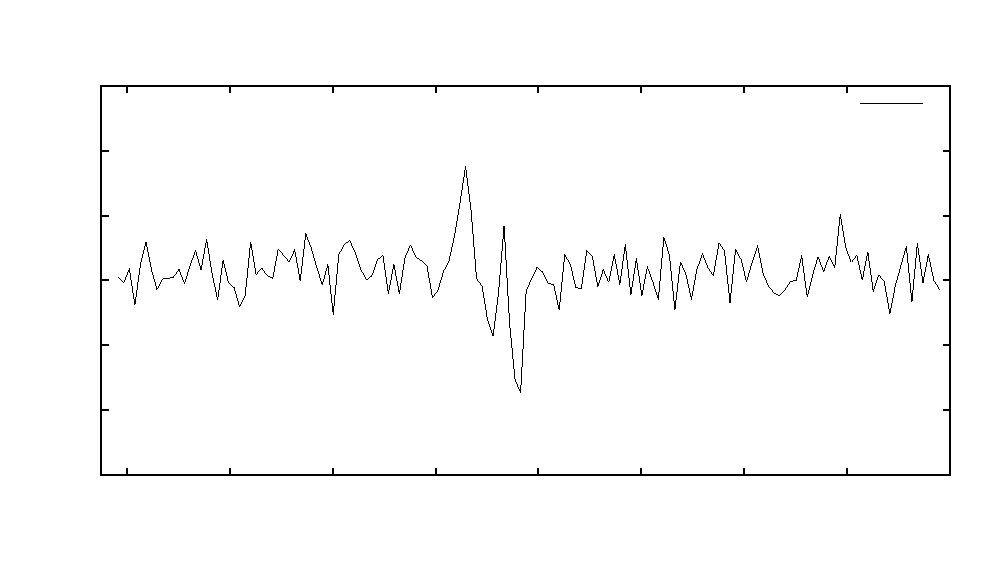
\includegraphics{ma03-12}}%
    \gplfronttext
  \end{picture}%
\endgroup

			\caption{\centering Parameter: Modulationsspannung 2V, AQ 30s, Empfindlichkeit 1mV, Phase 0^\circ}
		\end{figure}

		\begin{figure}[H]
			\center
			% GNUPLOT: LaTeX picture with Postscript
\begingroup
  \makeatletter
  \providecommand\color[2][]{%
    \GenericError{(gnuplot) \space\space\space\@spaces}{%
      Package color not loaded in conjunction with
      terminal option `colourtext'%
    }{See the gnuplot documentation for explanation.%
    }{Either use 'blacktext' in gnuplot or load the package
      color.sty in LaTeX.}%
    \renewcommand\color[2][]{}%
  }%
  \providecommand\includegraphics[2][]{%
    \GenericError{(gnuplot) \space\space\space\@spaces}{%
      Package graphicx or graphics not loaded%
    }{See the gnuplot documentation for explanation.%
    }{The gnuplot epslatex terminal needs graphicx.sty or graphics.sty.}%
    \renewcommand\includegraphics[2][]{}%
  }%
  \providecommand\rotatebox[2]{#2}%
  \@ifundefined{ifGPcolor}{%
    \newif\ifGPcolor
    \GPcolorfalse
  }{}%
  \@ifundefined{ifGPblacktext}{%
    \newif\ifGPblacktext
    \GPblacktexttrue
  }{}%
  % define a \g@addto@macro without @ in the name:
  \let\gplgaddtomacro\g@addto@macro
  % define empty templates for all commands taking text:
  \gdef\gplbacktext{}%
  \gdef\gplfronttext{}%
  \makeatother
  \ifGPblacktext
    % no textcolor at all
    \def\colorrgb#1{}%
    \def\colorgray#1{}%
  \else
    % gray or color?
    \ifGPcolor
      \def\colorrgb#1{\color[rgb]{#1}}%
      \def\colorgray#1{\color[gray]{#1}}%
      \expandafter\def\csname LTw\endcsname{\color{white}}%
      \expandafter\def\csname LTb\endcsname{\color{black}}%
      \expandafter\def\csname LTa\endcsname{\color{black}}%
      \expandafter\def\csname LT0\endcsname{\color[rgb]{1,0,0}}%
      \expandafter\def\csname LT1\endcsname{\color[rgb]{0,1,0}}%
      \expandafter\def\csname LT2\endcsname{\color[rgb]{0,0,1}}%
      \expandafter\def\csname LT3\endcsname{\color[rgb]{1,0,1}}%
      \expandafter\def\csname LT4\endcsname{\color[rgb]{0,1,1}}%
      \expandafter\def\csname LT5\endcsname{\color[rgb]{1,1,0}}%
      \expandafter\def\csname LT6\endcsname{\color[rgb]{0,0,0}}%
      \expandafter\def\csname LT7\endcsname{\color[rgb]{1,0.3,0}}%
      \expandafter\def\csname LT8\endcsname{\color[rgb]{0.5,0.5,0.5}}%
    \else
      % gray
      \def\colorrgb#1{\color{black}}%
      \def\colorgray#1{\color[gray]{#1}}%
      \expandafter\def\csname LTw\endcsname{\color{white}}%
      \expandafter\def\csname LTb\endcsname{\color{black}}%
      \expandafter\def\csname LTa\endcsname{\color{black}}%
      \expandafter\def\csname LT0\endcsname{\color{black}}%
      \expandafter\def\csname LT1\endcsname{\color{black}}%
      \expandafter\def\csname LT2\endcsname{\color{black}}%
      \expandafter\def\csname LT3\endcsname{\color{black}}%
      \expandafter\def\csname LT4\endcsname{\color{black}}%
      \expandafter\def\csname LT5\endcsname{\color{black}}%
      \expandafter\def\csname LT6\endcsname{\color{black}}%
      \expandafter\def\csname LT7\endcsname{\color{black}}%
      \expandafter\def\csname LT8\endcsname{\color{black}}%
    \fi
  \fi
  \setlength{\unitlength}{0.0500bp}%
  \begin{picture}(9354.00,5102.00)%
    \gplgaddtomacro\gplbacktext{%
      \csname LTb\endcsname%
      \put(682,704){\makebox(0,0)[r]{\strut{}-3}}%
      \put(682,1327){\makebox(0,0)[r]{\strut{}-2}}%
      \put(682,1950){\makebox(0,0)[r]{\strut{}-1}}%
      \put(682,2573){\makebox(0,0)[r]{\strut{} 0}}%
      \put(682,3195){\makebox(0,0)[r]{\strut{} 1}}%
      \put(682,3818){\makebox(0,0)[r]{\strut{} 2}}%
      \put(682,4441){\makebox(0,0)[r]{\strut{} 3}}%
      \put(1061,484){\makebox(0,0){\strut{} 280}}%
      \put(2048,484){\makebox(0,0){\strut{} 300}}%
      \put(3035,484){\makebox(0,0){\strut{} 320}}%
      \put(4022,484){\makebox(0,0){\strut{} 340}}%
      \put(5009,484){\makebox(0,0){\strut{} 360}}%
      \put(5996,484){\makebox(0,0){\strut{} 380}}%
      \put(6983,484){\makebox(0,0){\strut{} 400}}%
      \put(7970,484){\makebox(0,0){\strut{} 420}}%
      \put(8957,484){\makebox(0,0){\strut{} 440}}%
      \put(176,2572){\rotatebox{-270}{\makebox(0,0){\strut{}$dN/dE \ [1]$}}}%
      \put(4885,154){\makebox(0,0){\strut{}$E \ [eV]$}}%
      \put(4885,4771){\makebox(0,0){\strut{}Ag-Spektrum mit Zeitkonstante $300ms$}}%
    }%
    \gplgaddtomacro\gplfronttext{%
      \csname LTb\endcsname%
      \put(7970,4268){\makebox(0,0)[r]{\strut{}Messwerte}}%
    }%
    \gplbacktext
    \put(0,0){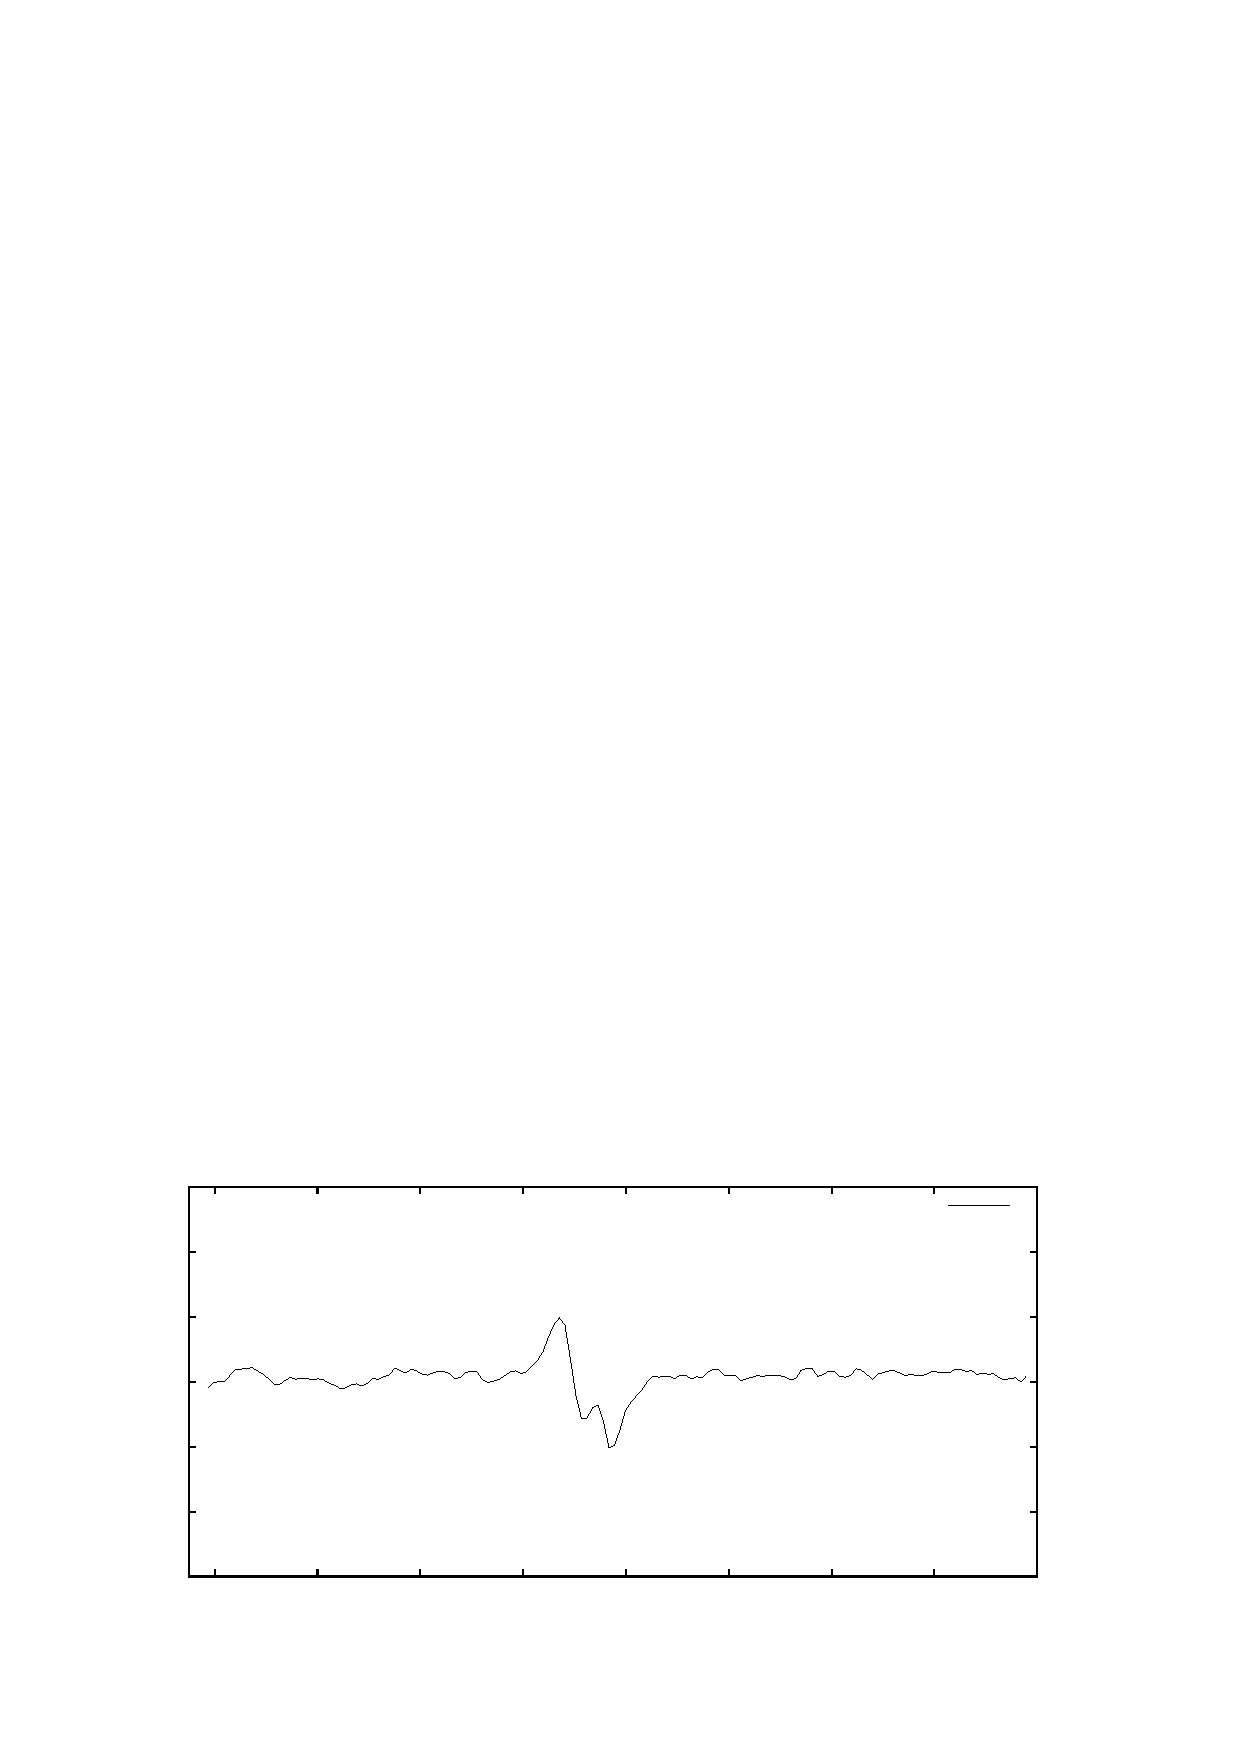
\includegraphics{ma03-11}}%
    \gplfronttext
  \end{picture}%
\endgroup

			\caption{\centering Parameter: Modulationsspannung 2V, AQ 30s, Empfindlichkeit 1mV, Phase 0^\circ}
		\end{figure}

		\begin{figure}[H]
			\center
			% GNUPLOT: LaTeX picture with Postscript
\begingroup
  \makeatletter
  \providecommand\color[2][]{%
    \GenericError{(gnuplot) \space\space\space\@spaces}{%
      Package color not loaded in conjunction with
      terminal option `colourtext'%
    }{See the gnuplot documentation for explanation.%
    }{Either use 'blacktext' in gnuplot or load the package
      color.sty in LaTeX.}%
    \renewcommand\color[2][]{}%
  }%
  \providecommand\includegraphics[2][]{%
    \GenericError{(gnuplot) \space\space\space\@spaces}{%
      Package graphicx or graphics not loaded%
    }{See the gnuplot documentation for explanation.%
    }{The gnuplot epslatex terminal needs graphicx.sty or graphics.sty.}%
    \renewcommand\includegraphics[2][]{}%
  }%
  \providecommand\rotatebox[2]{#2}%
  \@ifundefined{ifGPcolor}{%
    \newif\ifGPcolor
    \GPcolorfalse
  }{}%
  \@ifundefined{ifGPblacktext}{%
    \newif\ifGPblacktext
    \GPblacktexttrue
  }{}%
  % define a \g@addto@macro without @ in the name:
  \let\gplgaddtomacro\g@addto@macro
  % define empty templates for all commands taking text:
  \gdef\gplbacktext{}%
  \gdef\gplfronttext{}%
  \makeatother
  \ifGPblacktext
    % no textcolor at all
    \def\colorrgb#1{}%
    \def\colorgray#1{}%
  \else
    % gray or color?
    \ifGPcolor
      \def\colorrgb#1{\color[rgb]{#1}}%
      \def\colorgray#1{\color[gray]{#1}}%
      \expandafter\def\csname LTw\endcsname{\color{white}}%
      \expandafter\def\csname LTb\endcsname{\color{black}}%
      \expandafter\def\csname LTa\endcsname{\color{black}}%
      \expandafter\def\csname LT0\endcsname{\color[rgb]{1,0,0}}%
      \expandafter\def\csname LT1\endcsname{\color[rgb]{0,1,0}}%
      \expandafter\def\csname LT2\endcsname{\color[rgb]{0,0,1}}%
      \expandafter\def\csname LT3\endcsname{\color[rgb]{1,0,1}}%
      \expandafter\def\csname LT4\endcsname{\color[rgb]{0,1,1}}%
      \expandafter\def\csname LT5\endcsname{\color[rgb]{1,1,0}}%
      \expandafter\def\csname LT6\endcsname{\color[rgb]{0,0,0}}%
      \expandafter\def\csname LT7\endcsname{\color[rgb]{1,0.3,0}}%
      \expandafter\def\csname LT8\endcsname{\color[rgb]{0.5,0.5,0.5}}%
    \else
      % gray
      \def\colorrgb#1{\color{black}}%
      \def\colorgray#1{\color[gray]{#1}}%
      \expandafter\def\csname LTw\endcsname{\color{white}}%
      \expandafter\def\csname LTb\endcsname{\color{black}}%
      \expandafter\def\csname LTa\endcsname{\color{black}}%
      \expandafter\def\csname LT0\endcsname{\color{black}}%
      \expandafter\def\csname LT1\endcsname{\color{black}}%
      \expandafter\def\csname LT2\endcsname{\color{black}}%
      \expandafter\def\csname LT3\endcsname{\color{black}}%
      \expandafter\def\csname LT4\endcsname{\color{black}}%
      \expandafter\def\csname LT5\endcsname{\color{black}}%
      \expandafter\def\csname LT6\endcsname{\color{black}}%
      \expandafter\def\csname LT7\endcsname{\color{black}}%
      \expandafter\def\csname LT8\endcsname{\color{black}}%
    \fi
  \fi
  \setlength{\unitlength}{0.0500bp}%
  \begin{picture}(9354.00,5102.00)%
    \gplgaddtomacro\gplbacktext{%
      \csname LTb\endcsname%
      \put(682,704){\makebox(0,0)[r]{\strut{}-3}}%
      \put(682,1327){\makebox(0,0)[r]{\strut{}-2}}%
      \put(682,1950){\makebox(0,0)[r]{\strut{}-1}}%
      \put(682,2573){\makebox(0,0)[r]{\strut{} 0}}%
      \put(682,3195){\makebox(0,0)[r]{\strut{} 1}}%
      \put(682,3818){\makebox(0,0)[r]{\strut{} 2}}%
      \put(682,4441){\makebox(0,0)[r]{\strut{} 3}}%
      \put(1061,484){\makebox(0,0){\strut{} 280}}%
      \put(2048,484){\makebox(0,0){\strut{} 300}}%
      \put(3035,484){\makebox(0,0){\strut{} 320}}%
      \put(4022,484){\makebox(0,0){\strut{} 340}}%
      \put(5009,484){\makebox(0,0){\strut{} 360}}%
      \put(5996,484){\makebox(0,0){\strut{} 380}}%
      \put(6983,484){\makebox(0,0){\strut{} 400}}%
      \put(7970,484){\makebox(0,0){\strut{} 420}}%
      \put(8957,484){\makebox(0,0){\strut{} 440}}%
      \put(176,2572){\rotatebox{-270}{\makebox(0,0){\strut{}$dN/dE \ [1]$}}}%
      \put(4885,154){\makebox(0,0){\strut{}$E \ [eV]$}}%
      \put(4885,4771){\makebox(0,0){\strut{}Ag-Spektrum mit Zeitkonstante $1000ms$}}%
    }%
    \gplgaddtomacro\gplfronttext{%
      \csname LTb\endcsname%
      \put(7970,4268){\makebox(0,0)[r]{\strut{}Messwerte}}%
    }%
    \gplbacktext
    \put(0,0){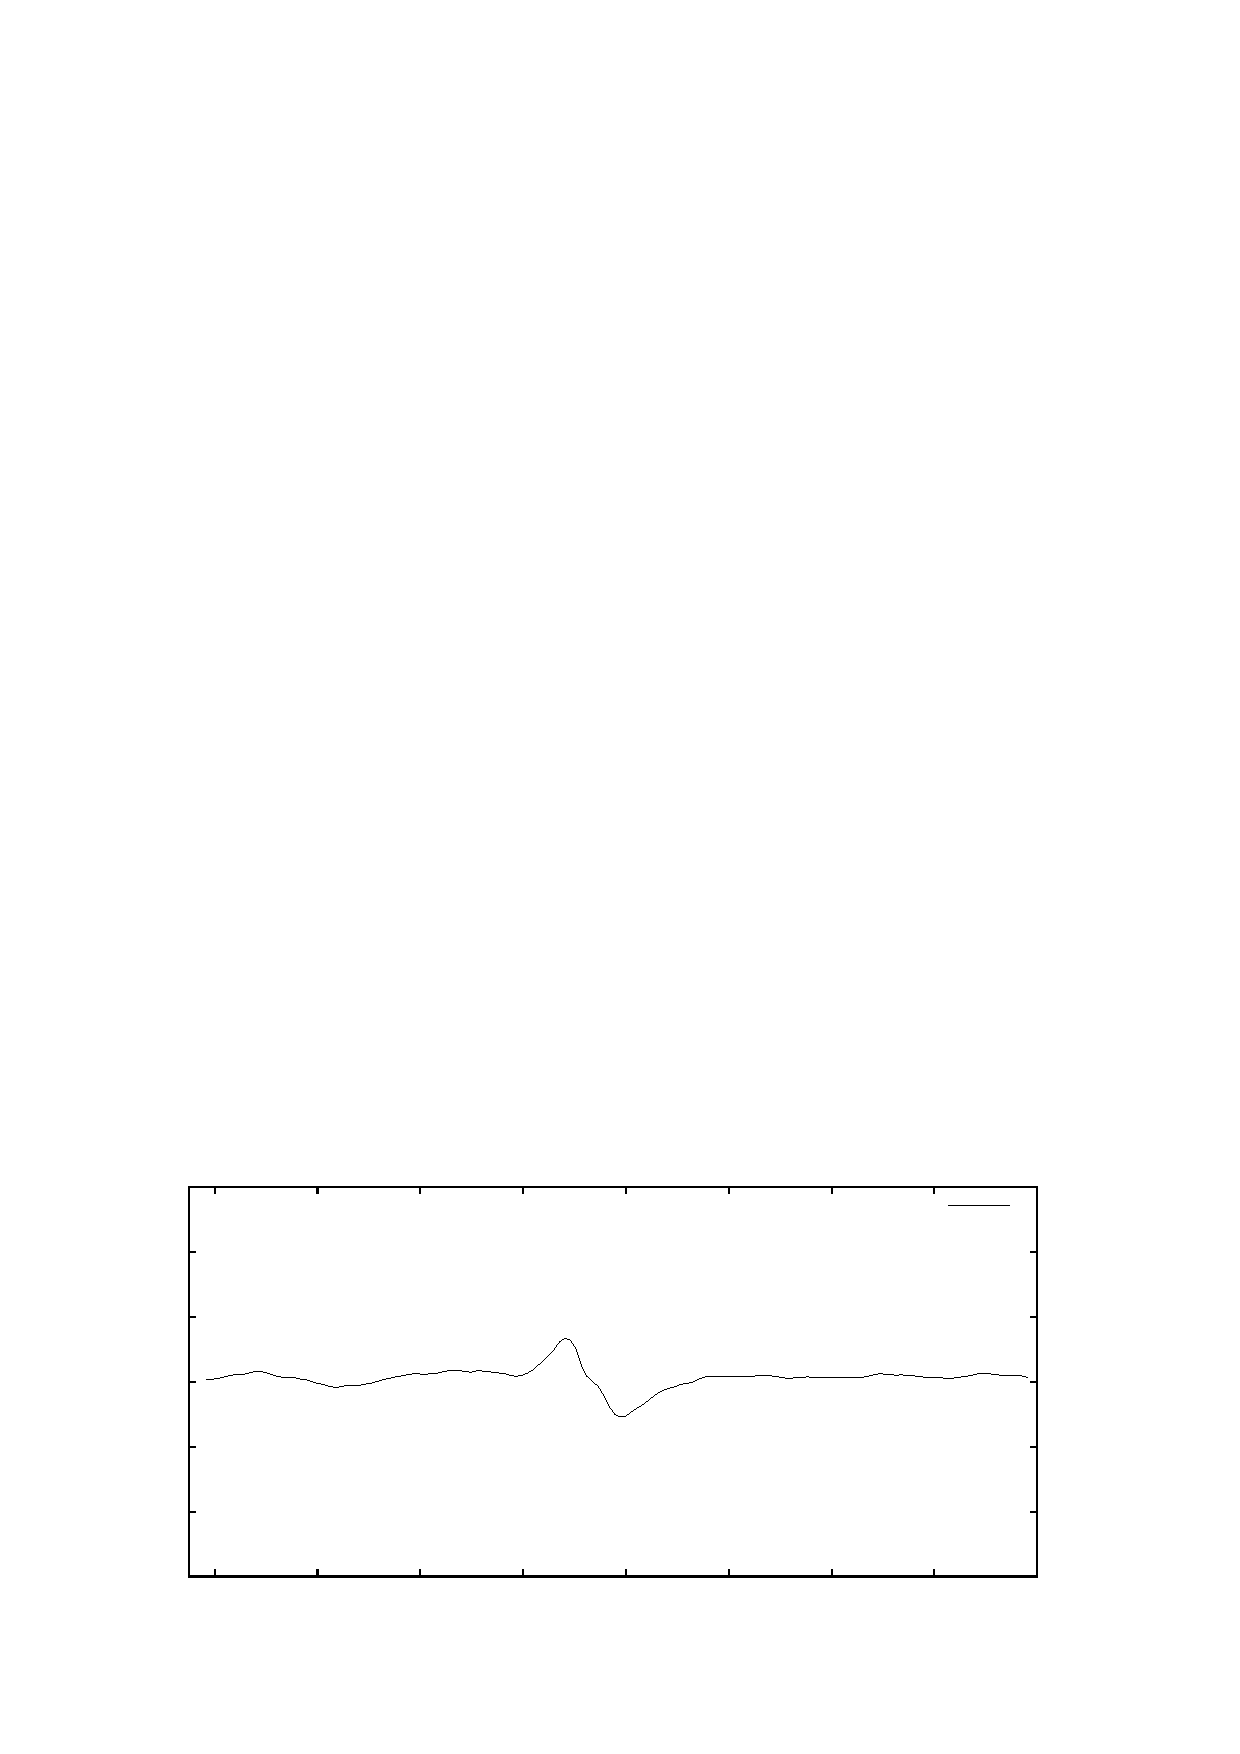
\includegraphics{ma03-10}}%
    \gplfronttext
  \end{picture}%
\endgroup

			\caption{\centering Parameter: Modulationsspannung 2V, AQ 30s, Empfindlichkeit 1mV, Phase 0^\circ}
		\end{figure}

		Es ist nun erkennbar, dass durch die zeitliche Mittelung ein besseres Signal-Rausch-Verhältnis erlangt werden kann.
		Wählt man die Zeitkonstante jedoch zu groß, so wird das Auflösungsvermögen drastisch verringert. Eine einfache Rechnung zeigt, über wie viel Elektronenvolt gemittelt wird:

		\begin{equation*}
			\Delta E = \dfrac{\Delta U_{CMA} \cdot K \cdot \text{\itshape Zeitkonstante}}{\text{\itshape Aquirationtime}}
		\end{equation*}
	

		Spannungsbereich und Aquirationtime wurden bei den drei Aufnahmen nicht verändert.
		\begin{equation*}
			\dfrac{\Delta U_{CMA} \cdot K}{\text{\itshape Aquirationtime}} = \dfrac{200V \cdot 1.624}{30s} \approx 10.8 \dfrac{V}{s}
		\end{equation*}
		\begin{itemize}
			\item 
				$10.8 Vs^{-1} \cdot 10ms = 108mV$
			\item 
				$10.8 Vs^{-1} \cdot 300ms = 3.25V$
			\item 
				$10.8 Vs^{-1} \cdot 1000ms = 10.8V$
		\end{itemize}
		Demnach ist es auch plausibel, dass der Doppelpeak bei 10 und 300ms Zeitkonstante noch zu erkennen war, wogegen er bei 1000ms verschwimmt.

	% subsubsection zeitkonstante (end)

	\subsubsection{Phase} % (fold)
	\label{ssub:phase}
	
		\begin{figure}[H]
			\center
			% GNUPLOT: LaTeX picture with Postscript
\begingroup
  \makeatletter
  \providecommand\color[2][]{%
    \GenericError{(gnuplot) \space\space\space\@spaces}{%
      Package color not loaded in conjunction with
      terminal option `colourtext'%
    }{See the gnuplot documentation for explanation.%
    }{Either use 'blacktext' in gnuplot or load the package
      color.sty in LaTeX.}%
    \renewcommand\color[2][]{}%
  }%
  \providecommand\includegraphics[2][]{%
    \GenericError{(gnuplot) \space\space\space\@spaces}{%
      Package graphicx or graphics not loaded%
    }{See the gnuplot documentation for explanation.%
    }{The gnuplot epslatex terminal needs graphicx.sty or graphics.sty.}%
    \renewcommand\includegraphics[2][]{}%
  }%
  \providecommand\rotatebox[2]{#2}%
  \@ifundefined{ifGPcolor}{%
    \newif\ifGPcolor
    \GPcolorfalse
  }{}%
  \@ifundefined{ifGPblacktext}{%
    \newif\ifGPblacktext
    \GPblacktexttrue
  }{}%
  % define a \g@addto@macro without @ in the name:
  \let\gplgaddtomacro\g@addto@macro
  % define empty templates for all commands taking text:
  \gdef\gplbacktext{}%
  \gdef\gplfronttext{}%
  \makeatother
  \ifGPblacktext
    % no textcolor at all
    \def\colorrgb#1{}%
    \def\colorgray#1{}%
  \else
    % gray or color?
    \ifGPcolor
      \def\colorrgb#1{\color[rgb]{#1}}%
      \def\colorgray#1{\color[gray]{#1}}%
      \expandafter\def\csname LTw\endcsname{\color{white}}%
      \expandafter\def\csname LTb\endcsname{\color{black}}%
      \expandafter\def\csname LTa\endcsname{\color{black}}%
      \expandafter\def\csname LT0\endcsname{\color[rgb]{1,0,0}}%
      \expandafter\def\csname LT1\endcsname{\color[rgb]{0,1,0}}%
      \expandafter\def\csname LT2\endcsname{\color[rgb]{0,0,1}}%
      \expandafter\def\csname LT3\endcsname{\color[rgb]{1,0,1}}%
      \expandafter\def\csname LT4\endcsname{\color[rgb]{0,1,1}}%
      \expandafter\def\csname LT5\endcsname{\color[rgb]{1,1,0}}%
      \expandafter\def\csname LT6\endcsname{\color[rgb]{0,0,0}}%
      \expandafter\def\csname LT7\endcsname{\color[rgb]{1,0.3,0}}%
      \expandafter\def\csname LT8\endcsname{\color[rgb]{0.5,0.5,0.5}}%
    \else
      % gray
      \def\colorrgb#1{\color{black}}%
      \def\colorgray#1{\color[gray]{#1}}%
      \expandafter\def\csname LTw\endcsname{\color{white}}%
      \expandafter\def\csname LTb\endcsname{\color{black}}%
      \expandafter\def\csname LTa\endcsname{\color{black}}%
      \expandafter\def\csname LT0\endcsname{\color{black}}%
      \expandafter\def\csname LT1\endcsname{\color{black}}%
      \expandafter\def\csname LT2\endcsname{\color{black}}%
      \expandafter\def\csname LT3\endcsname{\color{black}}%
      \expandafter\def\csname LT4\endcsname{\color{black}}%
      \expandafter\def\csname LT5\endcsname{\color{black}}%
      \expandafter\def\csname LT6\endcsname{\color{black}}%
      \expandafter\def\csname LT7\endcsname{\color{black}}%
      \expandafter\def\csname LT8\endcsname{\color{black}}%
    \fi
  \fi
  \setlength{\unitlength}{0.0500bp}%
  \begin{picture}(9354.00,5102.00)%
    \gplgaddtomacro\gplbacktext{%
      \csname LTb\endcsname%
      \put(946,704){\makebox(0,0)[r]{\strut{}-2}}%
      \put(946,1171){\makebox(0,0)[r]{\strut{}-1.5}}%
      \put(946,1638){\makebox(0,0)[r]{\strut{}-1}}%
      \put(946,2105){\makebox(0,0)[r]{\strut{}-0.5}}%
      \put(946,2573){\makebox(0,0)[r]{\strut{} 0}}%
      \put(946,3040){\makebox(0,0)[r]{\strut{} 0.5}}%
      \put(946,3507){\makebox(0,0)[r]{\strut{} 1}}%
      \put(946,3974){\makebox(0,0)[r]{\strut{} 1.5}}%
      \put(946,4441){\makebox(0,0)[r]{\strut{} 2}}%
      \put(1078,484){\makebox(0,0){\strut{} 310}}%
      \put(1953,484){\makebox(0,0){\strut{} 320}}%
      \put(2829,484){\makebox(0,0){\strut{} 330}}%
      \put(3704,484){\makebox(0,0){\strut{} 340}}%
      \put(4580,484){\makebox(0,0){\strut{} 350}}%
      \put(5455,484){\makebox(0,0){\strut{} 360}}%
      \put(6331,484){\makebox(0,0){\strut{} 370}}%
      \put(7206,484){\makebox(0,0){\strut{} 380}}%
      \put(8082,484){\makebox(0,0){\strut{} 390}}%
      \put(8957,484){\makebox(0,0){\strut{} 400}}%
      \put(176,2572){\rotatebox{-270}{\makebox(0,0){\strut{}$dN/dE \ [1]$}}}%
      \put(5017,154){\makebox(0,0){\strut{}$E \ [eV]$}}%
      \put(5017,4771){\makebox(0,0){\strut{}Ag-Spektrum mit Phase $45^\circ$}}%
    }%
    \gplgaddtomacro\gplfronttext{%
      \csname LTb\endcsname%
      \put(7970,4268){\makebox(0,0)[r]{\strut{}Messwerte}}%
    }%
    \gplbacktext
    \put(0,0){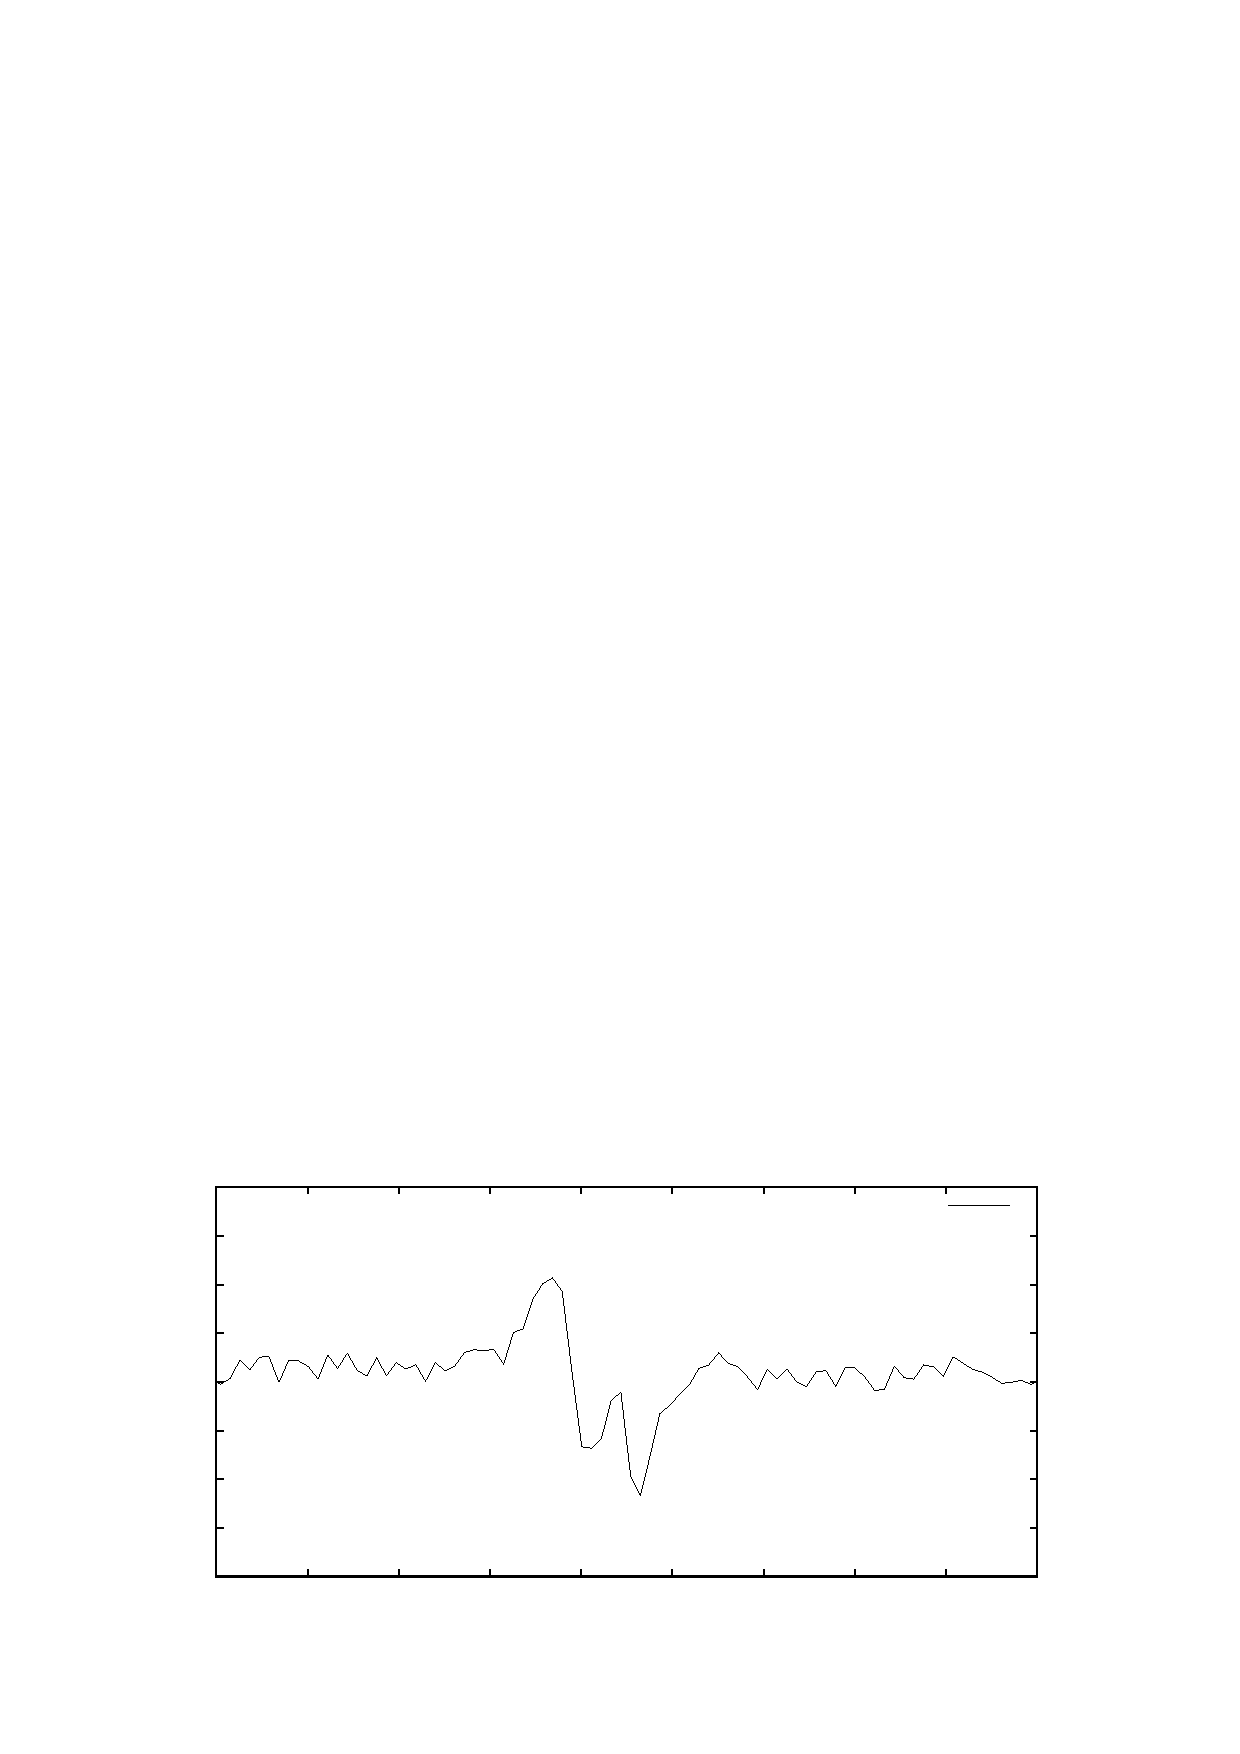
\includegraphics{ma03-08}}%
    \gplfronttext
  \end{picture}%
\endgroup

			\caption{\centering Parameter: Modulationsspannung 2V, AQ 30s, Empfindlichkeit 1mV, Zeitkonstante 100ms}
		\end{figure}

		\begin{figure}[H]
			\center
			% GNUPLOT: LaTeX picture with Postscript
\begingroup
  \makeatletter
  \providecommand\color[2][]{%
    \GenericError{(gnuplot) \space\space\space\@spaces}{%
      Package color not loaded in conjunction with
      terminal option `colourtext'%
    }{See the gnuplot documentation for explanation.%
    }{Either use 'blacktext' in gnuplot or load the package
      color.sty in LaTeX.}%
    \renewcommand\color[2][]{}%
  }%
  \providecommand\includegraphics[2][]{%
    \GenericError{(gnuplot) \space\space\space\@spaces}{%
      Package graphicx or graphics not loaded%
    }{See the gnuplot documentation for explanation.%
    }{The gnuplot epslatex terminal needs graphicx.sty or graphics.sty.}%
    \renewcommand\includegraphics[2][]{}%
  }%
  \providecommand\rotatebox[2]{#2}%
  \@ifundefined{ifGPcolor}{%
    \newif\ifGPcolor
    \GPcolorfalse
  }{}%
  \@ifundefined{ifGPblacktext}{%
    \newif\ifGPblacktext
    \GPblacktexttrue
  }{}%
  % define a \g@addto@macro without @ in the name:
  \let\gplgaddtomacro\g@addto@macro
  % define empty templates for all commands taking text:
  \gdef\gplbacktext{}%
  \gdef\gplfronttext{}%
  \makeatother
  \ifGPblacktext
    % no textcolor at all
    \def\colorrgb#1{}%
    \def\colorgray#1{}%
  \else
    % gray or color?
    \ifGPcolor
      \def\colorrgb#1{\color[rgb]{#1}}%
      \def\colorgray#1{\color[gray]{#1}}%
      \expandafter\def\csname LTw\endcsname{\color{white}}%
      \expandafter\def\csname LTb\endcsname{\color{black}}%
      \expandafter\def\csname LTa\endcsname{\color{black}}%
      \expandafter\def\csname LT0\endcsname{\color[rgb]{1,0,0}}%
      \expandafter\def\csname LT1\endcsname{\color[rgb]{0,1,0}}%
      \expandafter\def\csname LT2\endcsname{\color[rgb]{0,0,1}}%
      \expandafter\def\csname LT3\endcsname{\color[rgb]{1,0,1}}%
      \expandafter\def\csname LT4\endcsname{\color[rgb]{0,1,1}}%
      \expandafter\def\csname LT5\endcsname{\color[rgb]{1,1,0}}%
      \expandafter\def\csname LT6\endcsname{\color[rgb]{0,0,0}}%
      \expandafter\def\csname LT7\endcsname{\color[rgb]{1,0.3,0}}%
      \expandafter\def\csname LT8\endcsname{\color[rgb]{0.5,0.5,0.5}}%
    \else
      % gray
      \def\colorrgb#1{\color{black}}%
      \def\colorgray#1{\color[gray]{#1}}%
      \expandafter\def\csname LTw\endcsname{\color{white}}%
      \expandafter\def\csname LTb\endcsname{\color{black}}%
      \expandafter\def\csname LTa\endcsname{\color{black}}%
      \expandafter\def\csname LT0\endcsname{\color{black}}%
      \expandafter\def\csname LT1\endcsname{\color{black}}%
      \expandafter\def\csname LT2\endcsname{\color{black}}%
      \expandafter\def\csname LT3\endcsname{\color{black}}%
      \expandafter\def\csname LT4\endcsname{\color{black}}%
      \expandafter\def\csname LT5\endcsname{\color{black}}%
      \expandafter\def\csname LT6\endcsname{\color{black}}%
      \expandafter\def\csname LT7\endcsname{\color{black}}%
      \expandafter\def\csname LT8\endcsname{\color{black}}%
    \fi
  \fi
  \setlength{\unitlength}{0.0500bp}%
  \begin{picture}(9354.00,5102.00)%
    \gplgaddtomacro\gplbacktext{%
      \csname LTb\endcsname%
      \put(946,704){\makebox(0,0)[r]{\strut{}-2}}%
      \put(946,1171){\makebox(0,0)[r]{\strut{}-1.5}}%
      \put(946,1638){\makebox(0,0)[r]{\strut{}-1}}%
      \put(946,2105){\makebox(0,0)[r]{\strut{}-0.5}}%
      \put(946,2573){\makebox(0,0)[r]{\strut{} 0}}%
      \put(946,3040){\makebox(0,0)[r]{\strut{} 0.5}}%
      \put(946,3507){\makebox(0,0)[r]{\strut{} 1}}%
      \put(946,3974){\makebox(0,0)[r]{\strut{} 1.5}}%
      \put(946,4441){\makebox(0,0)[r]{\strut{} 2}}%
      \put(1078,484){\makebox(0,0){\strut{} 310}}%
      \put(1953,484){\makebox(0,0){\strut{} 320}}%
      \put(2829,484){\makebox(0,0){\strut{} 330}}%
      \put(3704,484){\makebox(0,0){\strut{} 340}}%
      \put(4580,484){\makebox(0,0){\strut{} 350}}%
      \put(5455,484){\makebox(0,0){\strut{} 360}}%
      \put(6331,484){\makebox(0,0){\strut{} 370}}%
      \put(7206,484){\makebox(0,0){\strut{} 380}}%
      \put(8082,484){\makebox(0,0){\strut{} 390}}%
      \put(8957,484){\makebox(0,0){\strut{} 400}}%
      \put(176,2572){\rotatebox{-270}{\makebox(0,0){\strut{}$dN/dE \ [1]$}}}%
      \put(5017,154){\makebox(0,0){\strut{}$E \ [eV]$}}%
      \put(5017,4771){\makebox(0,0){\strut{}Ag-Spektrum mit Phase $180^\circ$}}%
    }%
    \gplgaddtomacro\gplfronttext{%
      \csname LTb\endcsname%
      \put(7970,4268){\makebox(0,0)[r]{\strut{}Messwerte}}%
    }%
    \gplbacktext
    \put(0,0){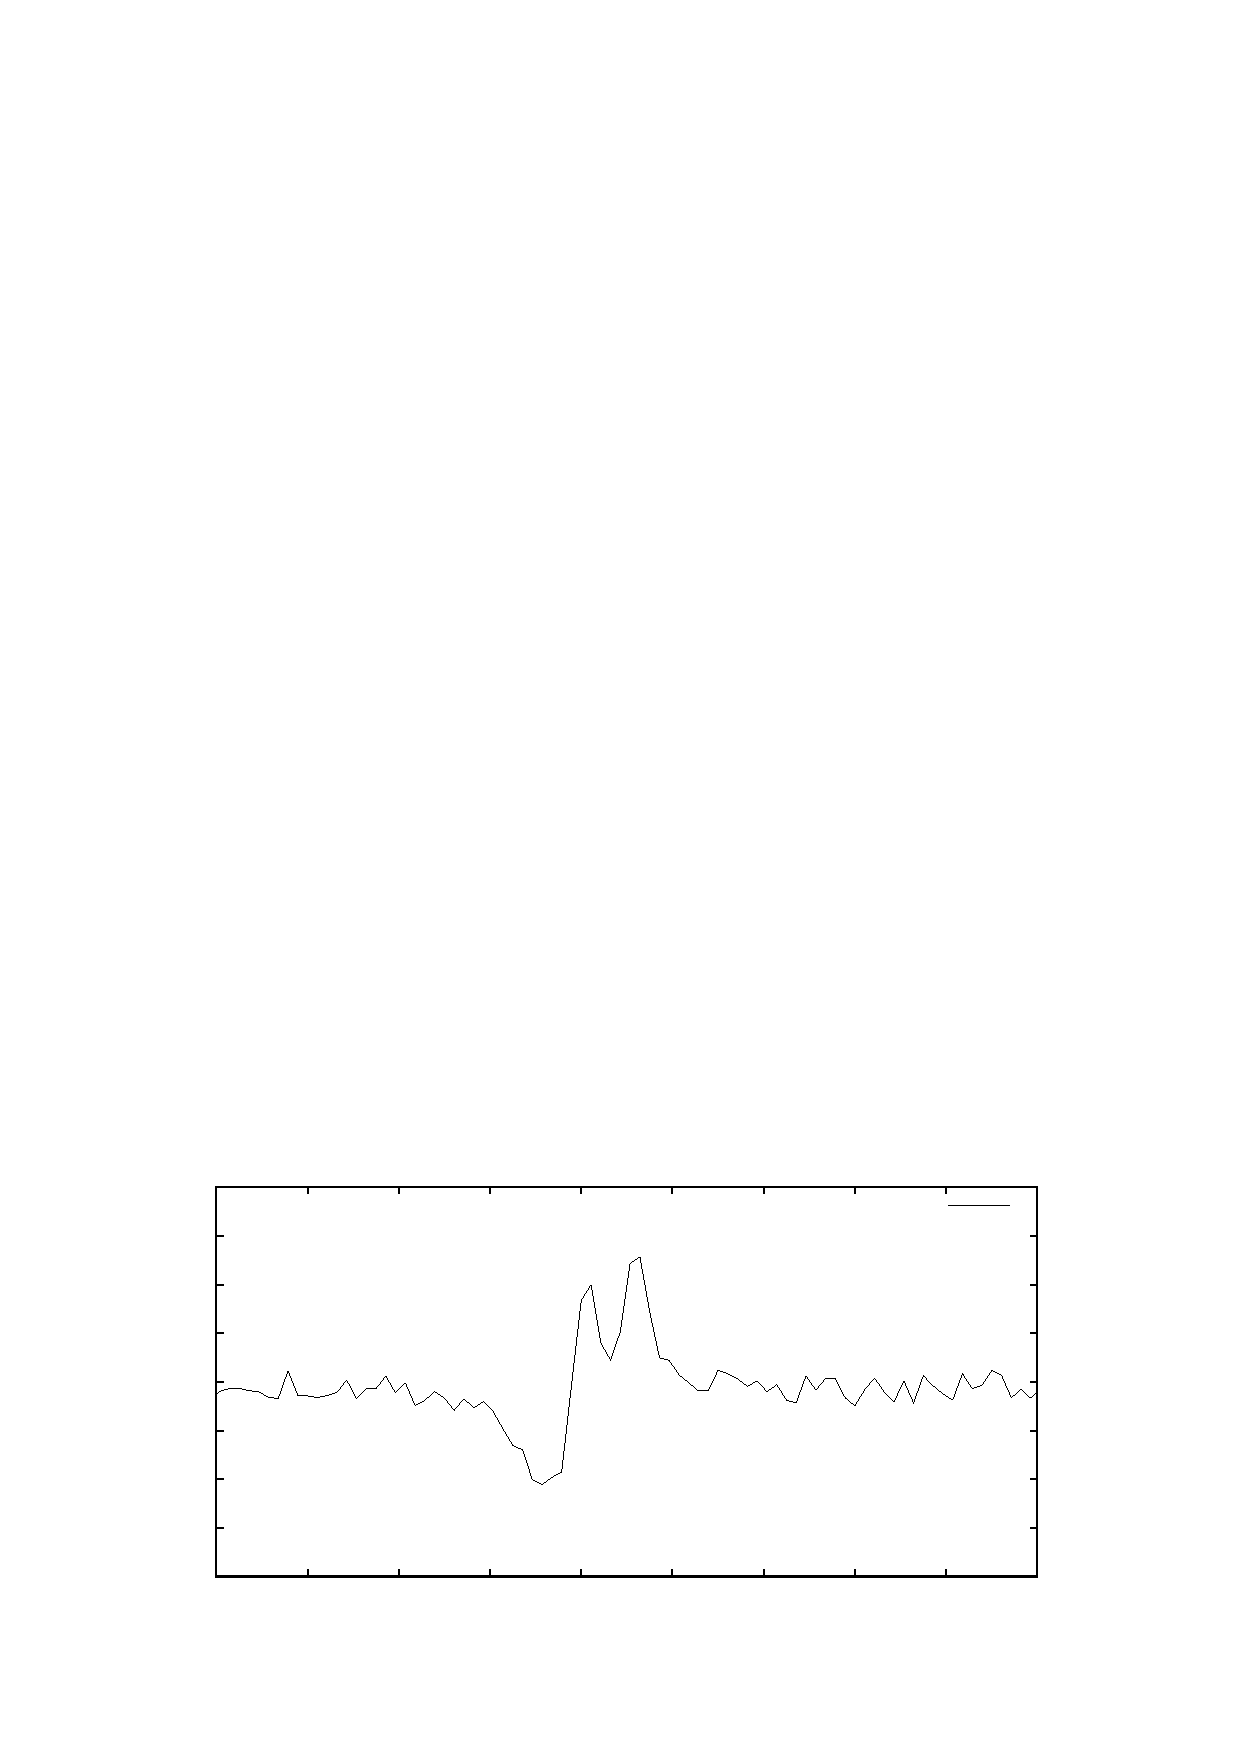
\includegraphics{ma03-07}}%
    \gplfronttext
  \end{picture}%
\endgroup

			\caption{\centering Parameter: Modulationsspannung 2V, AQ 30s, Empfindlichkeit 1mV, Zeitkonstante 100ms}
		\end{figure}

		\begin{figure}[H]
			\center
			% GNUPLOT: LaTeX picture with Postscript
\begingroup
  \makeatletter
  \providecommand\color[2][]{%
    \GenericError{(gnuplot) \space\space\space\@spaces}{%
      Package color not loaded in conjunction with
      terminal option `colourtext'%
    }{See the gnuplot documentation for explanation.%
    }{Either use 'blacktext' in gnuplot or load the package
      color.sty in LaTeX.}%
    \renewcommand\color[2][]{}%
  }%
  \providecommand\includegraphics[2][]{%
    \GenericError{(gnuplot) \space\space\space\@spaces}{%
      Package graphicx or graphics not loaded%
    }{See the gnuplot documentation for explanation.%
    }{The gnuplot epslatex terminal needs graphicx.sty or graphics.sty.}%
    \renewcommand\includegraphics[2][]{}%
  }%
  \providecommand\rotatebox[2]{#2}%
  \@ifundefined{ifGPcolor}{%
    \newif\ifGPcolor
    \GPcolorfalse
  }{}%
  \@ifundefined{ifGPblacktext}{%
    \newif\ifGPblacktext
    \GPblacktexttrue
  }{}%
  % define a \g@addto@macro without @ in the name:
  \let\gplgaddtomacro\g@addto@macro
  % define empty templates for all commands taking text:
  \gdef\gplbacktext{}%
  \gdef\gplfronttext{}%
  \makeatother
  \ifGPblacktext
    % no textcolor at all
    \def\colorrgb#1{}%
    \def\colorgray#1{}%
  \else
    % gray or color?
    \ifGPcolor
      \def\colorrgb#1{\color[rgb]{#1}}%
      \def\colorgray#1{\color[gray]{#1}}%
      \expandafter\def\csname LTw\endcsname{\color{white}}%
      \expandafter\def\csname LTb\endcsname{\color{black}}%
      \expandafter\def\csname LTa\endcsname{\color{black}}%
      \expandafter\def\csname LT0\endcsname{\color[rgb]{1,0,0}}%
      \expandafter\def\csname LT1\endcsname{\color[rgb]{0,1,0}}%
      \expandafter\def\csname LT2\endcsname{\color[rgb]{0,0,1}}%
      \expandafter\def\csname LT3\endcsname{\color[rgb]{1,0,1}}%
      \expandafter\def\csname LT4\endcsname{\color[rgb]{0,1,1}}%
      \expandafter\def\csname LT5\endcsname{\color[rgb]{1,1,0}}%
      \expandafter\def\csname LT6\endcsname{\color[rgb]{0,0,0}}%
      \expandafter\def\csname LT7\endcsname{\color[rgb]{1,0.3,0}}%
      \expandafter\def\csname LT8\endcsname{\color[rgb]{0.5,0.5,0.5}}%
    \else
      % gray
      \def\colorrgb#1{\color{black}}%
      \def\colorgray#1{\color[gray]{#1}}%
      \expandafter\def\csname LTw\endcsname{\color{white}}%
      \expandafter\def\csname LTb\endcsname{\color{black}}%
      \expandafter\def\csname LTa\endcsname{\color{black}}%
      \expandafter\def\csname LT0\endcsname{\color{black}}%
      \expandafter\def\csname LT1\endcsname{\color{black}}%
      \expandafter\def\csname LT2\endcsname{\color{black}}%
      \expandafter\def\csname LT3\endcsname{\color{black}}%
      \expandafter\def\csname LT4\endcsname{\color{black}}%
      \expandafter\def\csname LT5\endcsname{\color{black}}%
      \expandafter\def\csname LT6\endcsname{\color{black}}%
      \expandafter\def\csname LT7\endcsname{\color{black}}%
      \expandafter\def\csname LT8\endcsname{\color{black}}%
    \fi
  \fi
  \setlength{\unitlength}{0.0500bp}%
  \begin{picture}(9354.00,5102.00)%
    \gplgaddtomacro\gplbacktext{%
      \csname LTb\endcsname%
      \put(946,704){\makebox(0,0)[r]{\strut{}-2}}%
      \put(946,1171){\makebox(0,0)[r]{\strut{}-1.5}}%
      \put(946,1638){\makebox(0,0)[r]{\strut{}-1}}%
      \put(946,2105){\makebox(0,0)[r]{\strut{}-0.5}}%
      \put(946,2573){\makebox(0,0)[r]{\strut{} 0}}%
      \put(946,3040){\makebox(0,0)[r]{\strut{} 0.5}}%
      \put(946,3507){\makebox(0,0)[r]{\strut{} 1}}%
      \put(946,3974){\makebox(0,0)[r]{\strut{} 1.5}}%
      \put(946,4441){\makebox(0,0)[r]{\strut{} 2}}%
      \put(1078,484){\makebox(0,0){\strut{} 310}}%
      \put(1953,484){\makebox(0,0){\strut{} 320}}%
      \put(2829,484){\makebox(0,0){\strut{} 330}}%
      \put(3704,484){\makebox(0,0){\strut{} 340}}%
      \put(4580,484){\makebox(0,0){\strut{} 350}}%
      \put(5455,484){\makebox(0,0){\strut{} 360}}%
      \put(6331,484){\makebox(0,0){\strut{} 370}}%
      \put(7206,484){\makebox(0,0){\strut{} 380}}%
      \put(8082,484){\makebox(0,0){\strut{} 390}}%
      \put(8957,484){\makebox(0,0){\strut{} 400}}%
      \put(176,2572){\rotatebox{-270}{\makebox(0,0){\strut{}$dN/dE \ [1]$}}}%
      \put(5017,154){\makebox(0,0){\strut{}$E \ [eV]$}}%
      \put(5017,4771){\makebox(0,0){\strut{}Ag-Spektrum mit minimaler Phase bei $103^\circ$}}%
    }%
    \gplgaddtomacro\gplfronttext{%
      \csname LTb\endcsname%
      \put(7970,4268){\makebox(0,0)[r]{\strut{}Messwerte}}%
    }%
    \gplbacktext
    \put(0,0){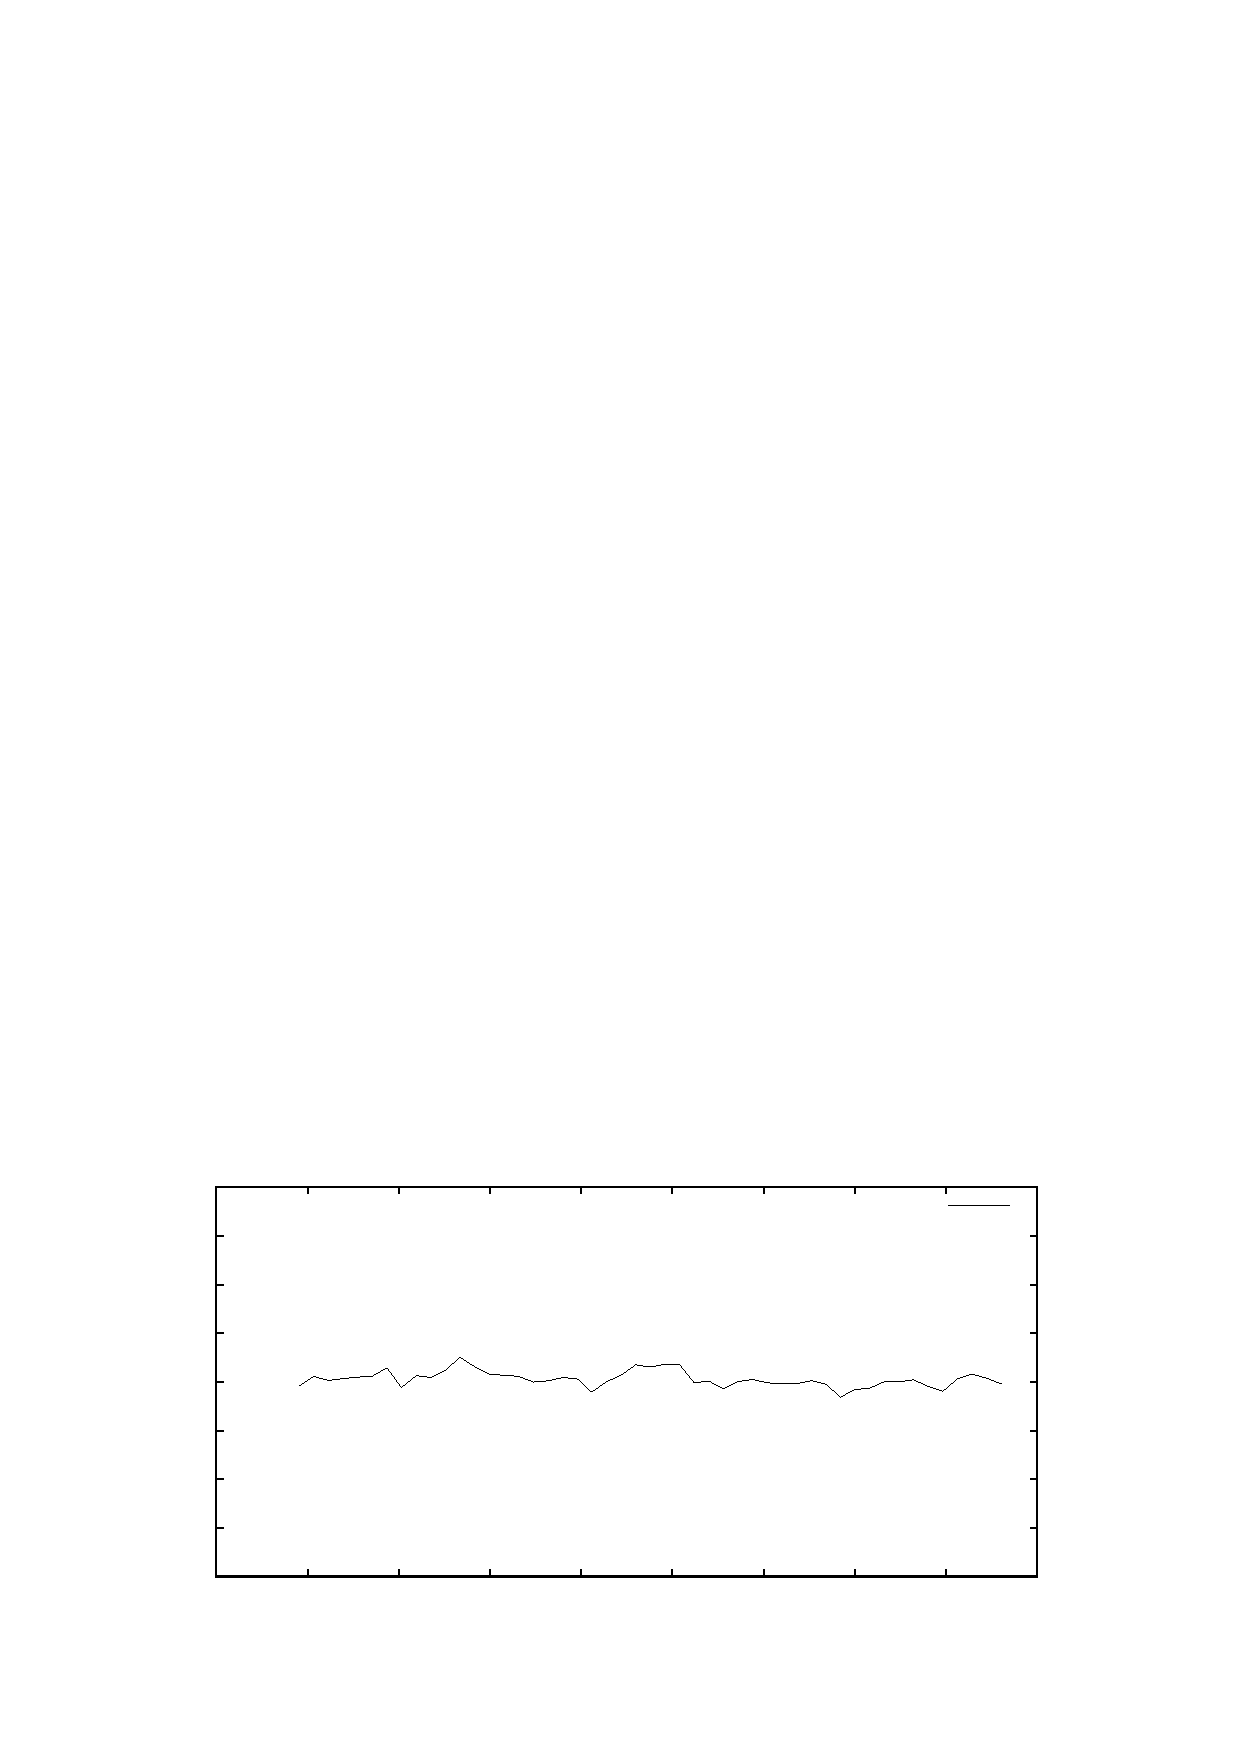
\includegraphics{ma03-14}}%
    \gplfronttext
  \end{picture}%
\endgroup

			\caption{\centering Parameter: Modulationsspannung 5V, AQ 10s, Empfindlichkeit 1mV, Zeitkonstante 300ms}
		\end{figure}

		Die Phasenverschiebung des Referenzsignals hat maßgeblich Einfluss auf die Amplitude des Signals, jedoch nicht oder kaum auf die Lage der Peaks. 
		Wie vermutet kehren sich bei einer Verschiebung in der Nähe von $180^\circ$ Minima und Maxima um. 
		Wenn man sich überlegt, wie zwei Sinusfunktionen im Demodulator multipliziert werden, so ergeben sie ohne Phasenverschiebung eine stets positive $\sin^2$-Funktion, mit einer Verschiebung von $180^\circ$ jedoch eine stets negative $–\sin^2$ Funktion. 
		Diese Überlegung macht den Vorzeichenwechsel plausibel. 
		Bei $103^\circ$ verschwand das Signal nahezu ganz. 
		Folglich muss der Phasenwinkel des maximalen Signals $90^\circ$ darunter liegen.
		Damit gilt also:
		\[
			\varphi_{max} = 13^\circ 
		\]
		Alle folgenden Spektren wurden mit einer Phasenverschiebung von $12^\circ$ aufgenommen.

	% subsubsection phase (end)

% subsection silber_spektrum (end)

\subsection{Analyse der Proben} % (fold)
\label{sub:qualitative_analyse_der_proben}

	\subsubsection{Probenhalter} % (fold)
	\label{ssub:probenhalter}
	
		\begin{figure}[H]
			\center
			% GNUPLOT: LaTeX picture with Postscript
\begingroup
  \makeatletter
  \providecommand\color[2][]{%
    \GenericError{(gnuplot) \space\space\space\@spaces}{%
      Package color not loaded in conjunction with
      terminal option `colourtext'%
    }{See the gnuplot documentation for explanation.%
    }{Either use 'blacktext' in gnuplot or load the package
      color.sty in LaTeX.}%
    \renewcommand\color[2][]{}%
  }%
  \providecommand\includegraphics[2][]{%
    \GenericError{(gnuplot) \space\space\space\@spaces}{%
      Package graphicx or graphics not loaded%
    }{See the gnuplot documentation for explanation.%
    }{The gnuplot epslatex terminal needs graphicx.sty or graphics.sty.}%
    \renewcommand\includegraphics[2][]{}%
  }%
  \providecommand\rotatebox[2]{#2}%
  \@ifundefined{ifGPcolor}{%
    \newif\ifGPcolor
    \GPcolorfalse
  }{}%
  \@ifundefined{ifGPblacktext}{%
    \newif\ifGPblacktext
    \GPblacktexttrue
  }{}%
  % define a \g@addto@macro without @ in the name:
  \let\gplgaddtomacro\g@addto@macro
  % define empty templates for all commands taking text:
  \gdef\gplbacktext{}%
  \gdef\gplfronttext{}%
  \makeatother
  \ifGPblacktext
    % no textcolor at all
    \def\colorrgb#1{}%
    \def\colorgray#1{}%
  \else
    % gray or color?
    \ifGPcolor
      \def\colorrgb#1{\color[rgb]{#1}}%
      \def\colorgray#1{\color[gray]{#1}}%
      \expandafter\def\csname LTw\endcsname{\color{white}}%
      \expandafter\def\csname LTb\endcsname{\color{black}}%
      \expandafter\def\csname LTa\endcsname{\color{black}}%
      \expandafter\def\csname LT0\endcsname{\color[rgb]{1,0,0}}%
      \expandafter\def\csname LT1\endcsname{\color[rgb]{0,1,0}}%
      \expandafter\def\csname LT2\endcsname{\color[rgb]{0,0,1}}%
      \expandafter\def\csname LT3\endcsname{\color[rgb]{1,0,1}}%
      \expandafter\def\csname LT4\endcsname{\color[rgb]{0,1,1}}%
      \expandafter\def\csname LT5\endcsname{\color[rgb]{1,1,0}}%
      \expandafter\def\csname LT6\endcsname{\color[rgb]{0,0,0}}%
      \expandafter\def\csname LT7\endcsname{\color[rgb]{1,0.3,0}}%
      \expandafter\def\csname LT8\endcsname{\color[rgb]{0.5,0.5,0.5}}%
    \else
      % gray
      \def\colorrgb#1{\color{black}}%
      \def\colorgray#1{\color[gray]{#1}}%
      \expandafter\def\csname LTw\endcsname{\color{white}}%
      \expandafter\def\csname LTb\endcsname{\color{black}}%
      \expandafter\def\csname LTa\endcsname{\color{black}}%
      \expandafter\def\csname LT0\endcsname{\color{black}}%
      \expandafter\def\csname LT1\endcsname{\color{black}}%
      \expandafter\def\csname LT2\endcsname{\color{black}}%
      \expandafter\def\csname LT3\endcsname{\color{black}}%
      \expandafter\def\csname LT4\endcsname{\color{black}}%
      \expandafter\def\csname LT5\endcsname{\color{black}}%
      \expandafter\def\csname LT6\endcsname{\color{black}}%
      \expandafter\def\csname LT7\endcsname{\color{black}}%
      \expandafter\def\csname LT8\endcsname{\color{black}}%
    \fi
  \fi
  \setlength{\unitlength}{0.0500bp}%
  \begin{picture}(9354.00,5668.00)%
    \gplgaddtomacro\gplbacktext{%
      \csname LTb\endcsname%
      \put(682,704){\makebox(0,0)[r]{\strut{}-6}}%
      \put(682,1421){\makebox(0,0)[r]{\strut{}-4}}%
      \put(682,2138){\makebox(0,0)[r]{\strut{}-2}}%
      \put(682,2856){\makebox(0,0)[r]{\strut{} 0}}%
      \put(682,3573){\makebox(0,0)[r]{\strut{} 2}}%
      \put(682,4290){\makebox(0,0)[r]{\strut{} 4}}%
      \put(682,5007){\makebox(0,0)[r]{\strut{} 6}}%
      \put(814,484){\makebox(0,0){\strut{} 0}}%
      \put(1719,484){\makebox(0,0){\strut{} 200}}%
      \put(2624,484){\makebox(0,0){\strut{} 400}}%
      \put(3528,484){\makebox(0,0){\strut{} 600}}%
      \put(4433,484){\makebox(0,0){\strut{} 800}}%
      \put(5338,484){\makebox(0,0){\strut{} 1000}}%
      \put(6243,484){\makebox(0,0){\strut{} 1200}}%
      \put(7147,484){\makebox(0,0){\strut{} 1400}}%
      \put(8052,484){\makebox(0,0){\strut{} 1600}}%
      \put(8957,484){\makebox(0,0){\strut{} 1800}}%
      \put(176,2855){\rotatebox{-270}{\makebox(0,0){\strut{}$dN/dE \ [1]$}}}%
      \put(4885,154){\makebox(0,0){\strut{}$E \ [eV]$}}%
      \put(4885,5337){\makebox(0,0){\strut{}Probenhalter-Spektrum an Position (2)}}%
      \put(6921,3035){\makebox(0,0)[l]{\strut{}1399}}%
      \put(3031,1600){\makebox(0,0)[l]{\strut{}520}}%
      \put(1809,2031){\makebox(0,0)[l]{\strut{}282}}%
    }%
    \gplgaddtomacro\gplfronttext{%
      \csname LTb\endcsname%
      \put(7970,4834){\makebox(0,0)[r]{\strut{}Messwerte}}%
    }%
    \gplbacktext
    \put(0,0){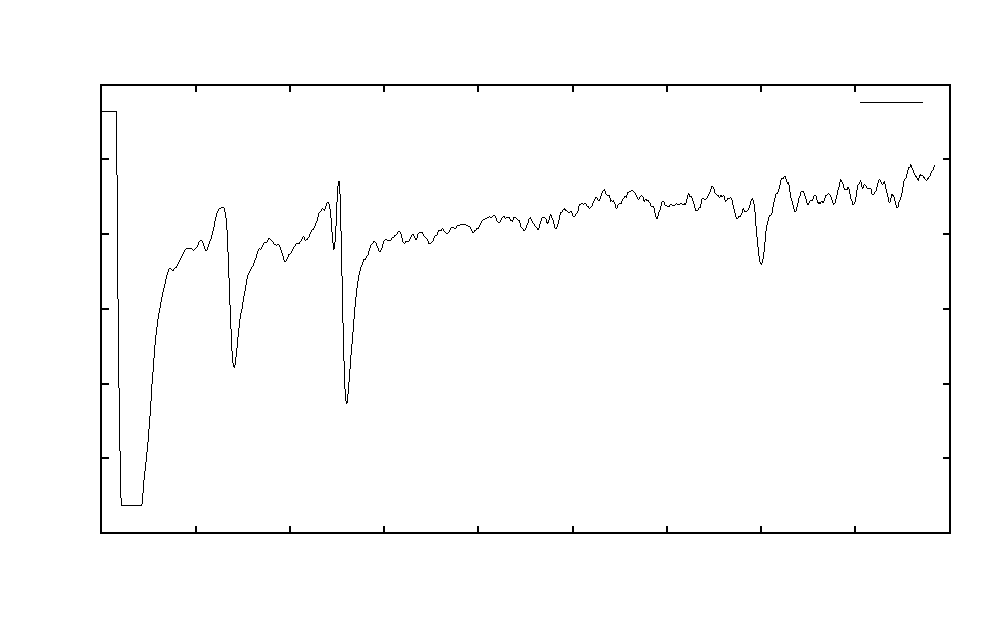
\includegraphics{ph2}}%
    \gplfronttext
  \end{picture}%
\endgroup

			\caption{\centering Parameter: Modulationsspannung 10V, AQ 6min, Empfindlichkeit 0.1mV, Zeitkonstante 3s, Phase 12^\circ}
		\end{figure}

		\begin{figure}[H]
			\center
			% GNUPLOT: LaTeX picture with Postscript
\begingroup
  \makeatletter
  \providecommand\color[2][]{%
    \GenericError{(gnuplot) \space\space\space\@spaces}{%
      Package color not loaded in conjunction with
      terminal option `colourtext'%
    }{See the gnuplot documentation for explanation.%
    }{Either use 'blacktext' in gnuplot or load the package
      color.sty in LaTeX.}%
    \renewcommand\color[2][]{}%
  }%
  \providecommand\includegraphics[2][]{%
    \GenericError{(gnuplot) \space\space\space\@spaces}{%
      Package graphicx or graphics not loaded%
    }{See the gnuplot documentation for explanation.%
    }{The gnuplot epslatex terminal needs graphicx.sty or graphics.sty.}%
    \renewcommand\includegraphics[2][]{}%
  }%
  \providecommand\rotatebox[2]{#2}%
  \@ifundefined{ifGPcolor}{%
    \newif\ifGPcolor
    \GPcolorfalse
  }{}%
  \@ifundefined{ifGPblacktext}{%
    \newif\ifGPblacktext
    \GPblacktexttrue
  }{}%
  % define a \g@addto@macro without @ in the name:
  \let\gplgaddtomacro\g@addto@macro
  % define empty templates for all commands taking text:
  \gdef\gplbacktext{}%
  \gdef\gplfronttext{}%
  \makeatother
  \ifGPblacktext
    % no textcolor at all
    \def\colorrgb#1{}%
    \def\colorgray#1{}%
  \else
    % gray or color?
    \ifGPcolor
      \def\colorrgb#1{\color[rgb]{#1}}%
      \def\colorgray#1{\color[gray]{#1}}%
      \expandafter\def\csname LTw\endcsname{\color{white}}%
      \expandafter\def\csname LTb\endcsname{\color{black}}%
      \expandafter\def\csname LTa\endcsname{\color{black}}%
      \expandafter\def\csname LT0\endcsname{\color[rgb]{1,0,0}}%
      \expandafter\def\csname LT1\endcsname{\color[rgb]{0,1,0}}%
      \expandafter\def\csname LT2\endcsname{\color[rgb]{0,0,1}}%
      \expandafter\def\csname LT3\endcsname{\color[rgb]{1,0,1}}%
      \expandafter\def\csname LT4\endcsname{\color[rgb]{0,1,1}}%
      \expandafter\def\csname LT5\endcsname{\color[rgb]{1,1,0}}%
      \expandafter\def\csname LT6\endcsname{\color[rgb]{0,0,0}}%
      \expandafter\def\csname LT7\endcsname{\color[rgb]{1,0.3,0}}%
      \expandafter\def\csname LT8\endcsname{\color[rgb]{0.5,0.5,0.5}}%
    \else
      % gray
      \def\colorrgb#1{\color{black}}%
      \def\colorgray#1{\color[gray]{#1}}%
      \expandafter\def\csname LTw\endcsname{\color{white}}%
      \expandafter\def\csname LTb\endcsname{\color{black}}%
      \expandafter\def\csname LTa\endcsname{\color{black}}%
      \expandafter\def\csname LT0\endcsname{\color{black}}%
      \expandafter\def\csname LT1\endcsname{\color{black}}%
      \expandafter\def\csname LT2\endcsname{\color{black}}%
      \expandafter\def\csname LT3\endcsname{\color{black}}%
      \expandafter\def\csname LT4\endcsname{\color{black}}%
      \expandafter\def\csname LT5\endcsname{\color{black}}%
      \expandafter\def\csname LT6\endcsname{\color{black}}%
      \expandafter\def\csname LT7\endcsname{\color{black}}%
      \expandafter\def\csname LT8\endcsname{\color{black}}%
    \fi
  \fi
  \setlength{\unitlength}{0.0500bp}%
  \begin{picture}(9354.00,5102.00)%
    \gplgaddtomacro\gplbacktext{%
      \csname LTb\endcsname%
      \put(682,704){\makebox(0,0)[r]{\strut{}-6}}%
      \put(682,1171){\makebox(0,0)[r]{\strut{}-5}}%
      \put(682,1638){\makebox(0,0)[r]{\strut{}-4}}%
      \put(682,2105){\makebox(0,0)[r]{\strut{}-3}}%
      \put(682,2573){\makebox(0,0)[r]{\strut{}-2}}%
      \put(682,3040){\makebox(0,0)[r]{\strut{}-1}}%
      \put(682,3507){\makebox(0,0)[r]{\strut{} 0}}%
      \put(682,3974){\makebox(0,0)[r]{\strut{} 1}}%
      \put(682,4441){\makebox(0,0)[r]{\strut{} 2}}%
      \put(814,484){\makebox(0,0){\strut{} 0}}%
      \put(1900,484){\makebox(0,0){\strut{} 20}}%
      \put(2985,484){\makebox(0,0){\strut{} 40}}%
      \put(4071,484){\makebox(0,0){\strut{} 60}}%
      \put(5157,484){\makebox(0,0){\strut{} 80}}%
      \put(6243,484){\makebox(0,0){\strut{} 100}}%
      \put(7328,484){\makebox(0,0){\strut{} 120}}%
      \put(8414,484){\makebox(0,0){\strut{} 140}}%
      \put(176,2572){\rotatebox{-270}{\makebox(0,0){\strut{}$dN/dE \ [1]$}}}%
      \put(4885,154){\makebox(0,0){\strut{}$E \ [eV]$}}%
      \put(4885,4771){\makebox(0,0){\strut{}Probenhalter-Spektrum an Position (2)}}%
      \put(4505,1078){\makebox(0,0)[l]{\strut{}68}}%
    }%
    \gplgaddtomacro\gplfronttext{%
      \csname LTb\endcsname%
      \put(7970,4268){\makebox(0,0)[r]{\strut{}Messwerte}}%
    }%
    \gplbacktext
    \put(0,0){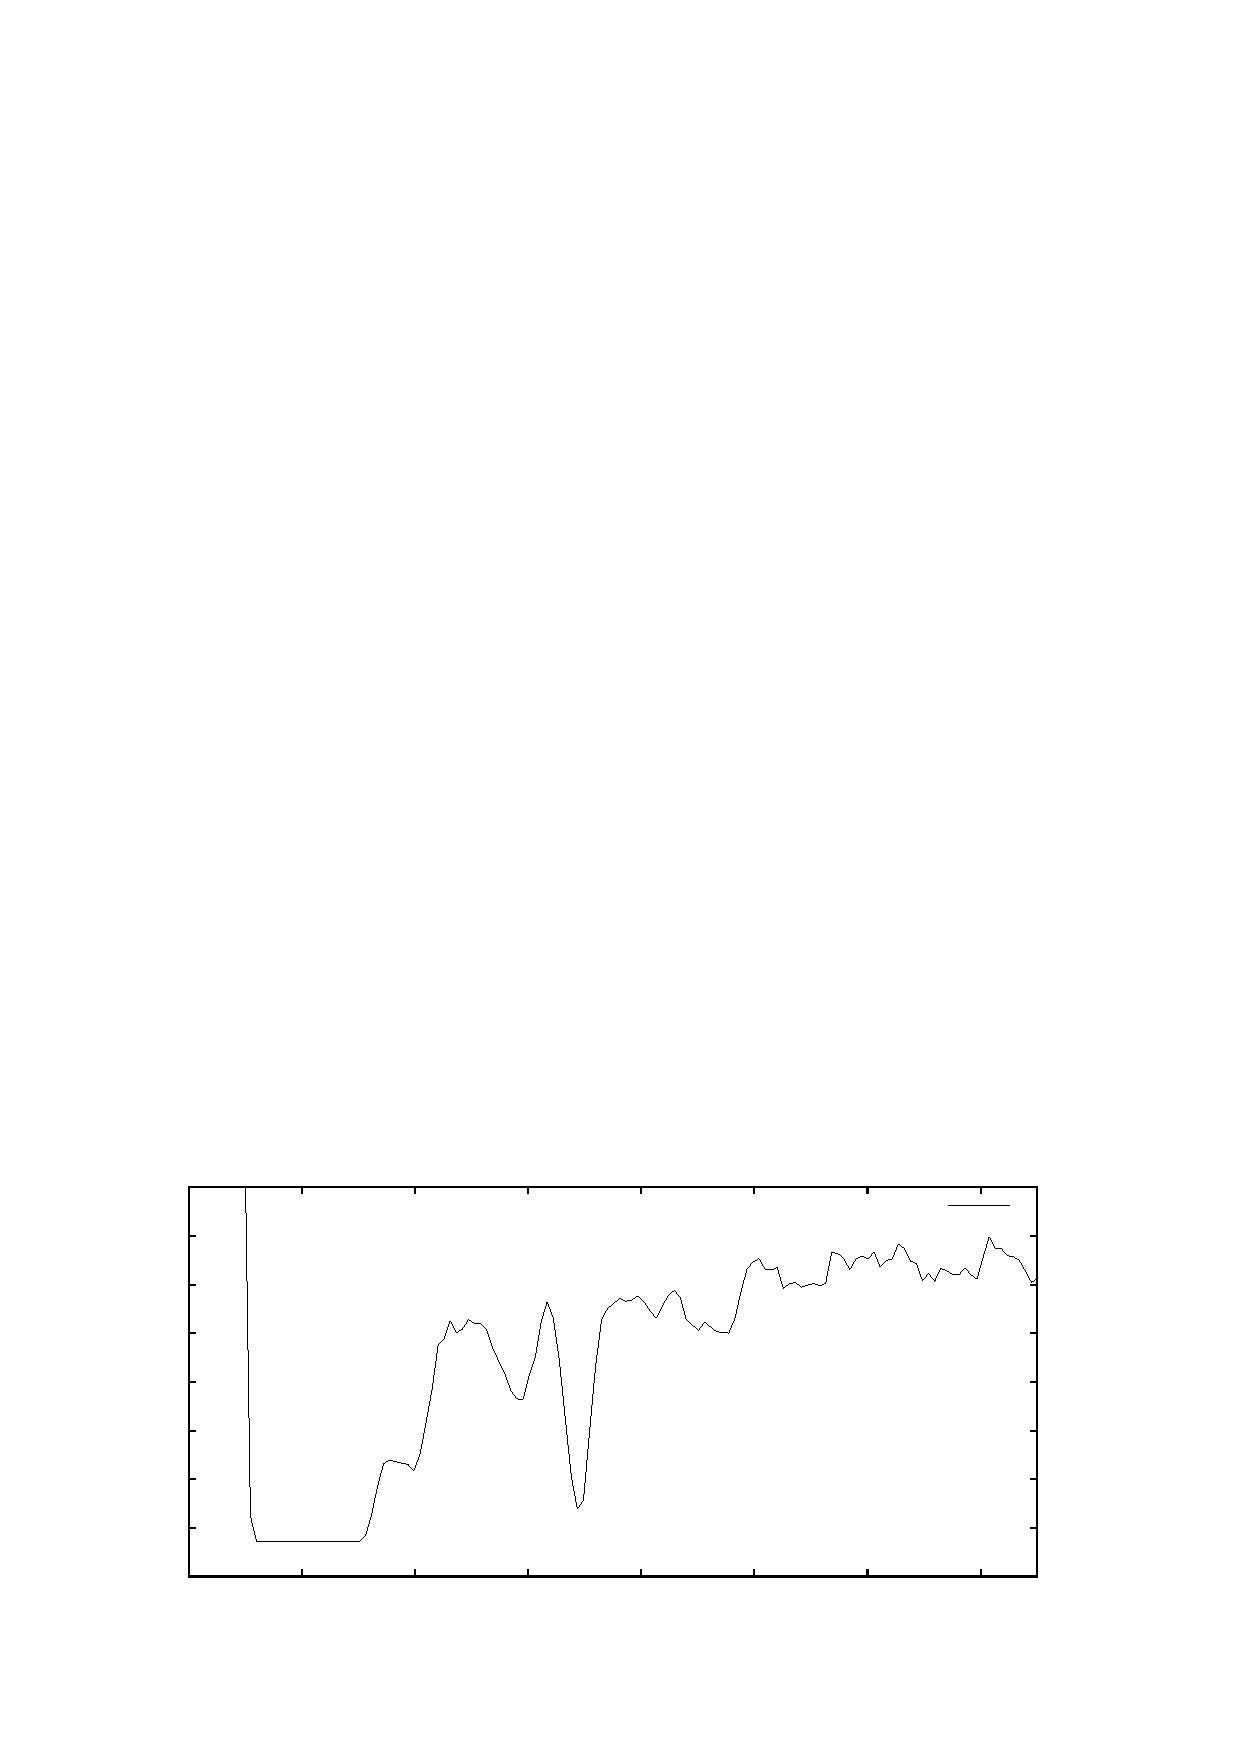
\includegraphics{ph4}}%
    \gplfronttext
  \end{picture}%
\endgroup

			\caption{\centering Parameter: Modulationsspannung 5V, AQ 60s, Empfindlichkeit 0.3mV, Zeitkonstante 300ms, Phase 12^\circ}
		\end{figure}

		Das erste Spektrum des Probenhalters zeigt drei ausgeprägte Minima.
		Diese wurden durch ein selbstgeschriebenes Programm ermittelt, wobei die jeweiligen Ergebnisse unterhalb der jeweiligen Peaks im Spektrum eingetragen wurden.
		Um auch den übersteuerten niederenergetischen Bereich zu vermessen wurde ein weiteres Spektrum mit geringerer Empfindlichkeit gemessen.

		Auch hier wurde der markanteste Peak markiert.
		Durch Vergleiche mit bereits vorhandenen Spektren aus \cite{handbook} (siehe Anhang), konnten folgende Elemente mit den jeweiligen Peak-Peak-Intensitäten nachgewiesen werden:

		\begin{description}
			\item[Kohlenstoff (C):] $4.29$ bei $282$eV (chemische Verschiebung des Energieniveaus)
			\item[Sauerstoff (O):] $5.97$ bei $520$eV (chemische Verschiebung des Energieniveaus)
			\item[Aluminium (Al):] $1.76$ bei $1399$eV
			\item[Aluminium (Al):] $4.32$ bei $68$eV (nicht mit den anderen Werten vergleichbar)
		\end{description}

		Berechnung der relativen Konzentrationen am Beispiel von Kohlenstoff (relative Empfindlichkeitsfaktoren aus \cite{article} entnommen):

		\begin{eqnarray*}
			c(C) &=& \dfrac{I(C)/S(C)}{I(C)/S(C) + I(O)/S(O) + I(Al)/S(Al)} \\
				&& \\
				&=& \dfrac{4.29/0.14}{4.29/0.14 + 5.97/0.40 + 4.32/0.19} \\
				&& \\
				&=& 0.55
		\end{eqnarray*}

		Analog folgt für alle gefundenen Elemente:
		\begin{itemize}
			\item 
				$c(C) = 0.55$
			\item
				$c(O) = 0.27$
			\item
				$c(Al) = 0.17$
		\end{itemize}

		Das Verhältnis von Aluminium zu Sauerstoff beträgt in etwa 2:3.
		Daraus lässt sich schließen, dass Aluminium und Sauerstoff in der Verbindung $Al_2O_3$ (Aluminiumoxid) an der Oberfläche vorkommen.
		Dies bestätigt, dass es sich bei dem Probenhalter um einen Großteil Aluminium handelt, da dieses an der Oberfläche immer eine Oxidschicht ausbildet.
		Aufgrund der chemischen Verschiebung des Kohlenstoff-Peaks ist zu erwarten, dass auch Kohlenstoff an der Oberfläche nur in gebundener Form vorliegt.
		Das hohe Vorkommen von Kohlenstoff deutet hier auf diverse Verunreinigungen des Probenhalters hin.

	% subsubsection probenhalter (end)

	\subsubsection{Probe 3} % (fold)
	\label{ssub:probe_3}
	
		\begin{figure}[H]
			\center
			% GNUPLOT: LaTeX picture with Postscript
\begingroup
  \makeatletter
  \providecommand\color[2][]{%
    \GenericError{(gnuplot) \space\space\space\@spaces}{%
      Package color not loaded in conjunction with
      terminal option `colourtext'%
    }{See the gnuplot documentation for explanation.%
    }{Either use 'blacktext' in gnuplot or load the package
      color.sty in LaTeX.}%
    \renewcommand\color[2][]{}%
  }%
  \providecommand\includegraphics[2][]{%
    \GenericError{(gnuplot) \space\space\space\@spaces}{%
      Package graphicx or graphics not loaded%
    }{See the gnuplot documentation for explanation.%
    }{The gnuplot epslatex terminal needs graphicx.sty or graphics.sty.}%
    \renewcommand\includegraphics[2][]{}%
  }%
  \providecommand\rotatebox[2]{#2}%
  \@ifundefined{ifGPcolor}{%
    \newif\ifGPcolor
    \GPcolorfalse
  }{}%
  \@ifundefined{ifGPblacktext}{%
    \newif\ifGPblacktext
    \GPblacktexttrue
  }{}%
  % define a \g@addto@macro without @ in the name:
  \let\gplgaddtomacro\g@addto@macro
  % define empty templates for all commands taking text:
  \gdef\gplbacktext{}%
  \gdef\gplfronttext{}%
  \makeatother
  \ifGPblacktext
    % no textcolor at all
    \def\colorrgb#1{}%
    \def\colorgray#1{}%
  \else
    % gray or color?
    \ifGPcolor
      \def\colorrgb#1{\color[rgb]{#1}}%
      \def\colorgray#1{\color[gray]{#1}}%
      \expandafter\def\csname LTw\endcsname{\color{white}}%
      \expandafter\def\csname LTb\endcsname{\color{black}}%
      \expandafter\def\csname LTa\endcsname{\color{black}}%
      \expandafter\def\csname LT0\endcsname{\color[rgb]{1,0,0}}%
      \expandafter\def\csname LT1\endcsname{\color[rgb]{0,1,0}}%
      \expandafter\def\csname LT2\endcsname{\color[rgb]{0,0,1}}%
      \expandafter\def\csname LT3\endcsname{\color[rgb]{1,0,1}}%
      \expandafter\def\csname LT4\endcsname{\color[rgb]{0,1,1}}%
      \expandafter\def\csname LT5\endcsname{\color[rgb]{1,1,0}}%
      \expandafter\def\csname LT6\endcsname{\color[rgb]{0,0,0}}%
      \expandafter\def\csname LT7\endcsname{\color[rgb]{1,0.3,0}}%
      \expandafter\def\csname LT8\endcsname{\color[rgb]{0.5,0.5,0.5}}%
    \else
      % gray
      \def\colorrgb#1{\color{black}}%
      \def\colorgray#1{\color[gray]{#1}}%
      \expandafter\def\csname LTw\endcsname{\color{white}}%
      \expandafter\def\csname LTb\endcsname{\color{black}}%
      \expandafter\def\csname LTa\endcsname{\color{black}}%
      \expandafter\def\csname LT0\endcsname{\color{black}}%
      \expandafter\def\csname LT1\endcsname{\color{black}}%
      \expandafter\def\csname LT2\endcsname{\color{black}}%
      \expandafter\def\csname LT3\endcsname{\color{black}}%
      \expandafter\def\csname LT4\endcsname{\color{black}}%
      \expandafter\def\csname LT5\endcsname{\color{black}}%
      \expandafter\def\csname LT6\endcsname{\color{black}}%
      \expandafter\def\csname LT7\endcsname{\color{black}}%
      \expandafter\def\csname LT8\endcsname{\color{black}}%
    \fi
  \fi
  \setlength{\unitlength}{0.0500bp}%
  \begin{picture}(9354.00,6802.00)%
    \gplgaddtomacro\gplbacktext{%
      \csname LTb\endcsname%
      \put(682,704){\makebox(0,0)[r]{\strut{}-4}}%
      \put(682,1248){\makebox(0,0)[r]{\strut{}-3}}%
      \put(682,1791){\makebox(0,0)[r]{\strut{}-2}}%
      \put(682,2335){\makebox(0,0)[r]{\strut{}-1}}%
      \put(682,2879){\makebox(0,0)[r]{\strut{} 0}}%
      \put(682,3423){\makebox(0,0)[r]{\strut{} 1}}%
      \put(682,3966){\makebox(0,0)[r]{\strut{} 2}}%
      \put(682,4510){\makebox(0,0)[r]{\strut{} 3}}%
      \put(682,5054){\makebox(0,0)[r]{\strut{} 4}}%
      \put(682,5597){\makebox(0,0)[r]{\strut{} 5}}%
      \put(682,6141){\makebox(0,0)[r]{\strut{} 6}}%
      \put(814,484){\makebox(0,0){\strut{} 0}}%
      \put(1719,484){\makebox(0,0){\strut{} 200}}%
      \put(2624,484){\makebox(0,0){\strut{} 400}}%
      \put(3528,484){\makebox(0,0){\strut{} 600}}%
      \put(4433,484){\makebox(0,0){\strut{} 800}}%
      \put(5338,484){\makebox(0,0){\strut{} 1000}}%
      \put(6243,484){\makebox(0,0){\strut{} 1200}}%
      \put(7147,484){\makebox(0,0){\strut{} 1400}}%
      \put(8052,484){\makebox(0,0){\strut{} 1600}}%
      \put(8957,484){\makebox(0,0){\strut{} 1800}}%
      \put(176,3422){\rotatebox{-270}{\makebox(0,0){\strut{}$dN/dE \ [1]$}}}%
      \put(4885,154){\makebox(0,0){\strut{}$E \ [eV]$}}%
      \put(4885,6471){\makebox(0,0){\strut{}Proben-Spektrum an Position (3)}}%
      \put(2081,2444){\makebox(0,0)[l]{\strut{}280}}%
      \put(1312,976){\makebox(0,0)[l]{\strut{}86}}%
      \put(3302,976){\makebox(0,0)[l]{\strut{}518}}%
      \put(8097,2988){\makebox(0,0)[l]{\strut{}1621}}%
    }%
    \gplgaddtomacro\gplfronttext{%
      \csname LTb\endcsname%
      \put(7970,5968){\makebox(0,0)[r]{\strut{}Messwerte}}%
    }%
    \gplbacktext
    \put(0,0){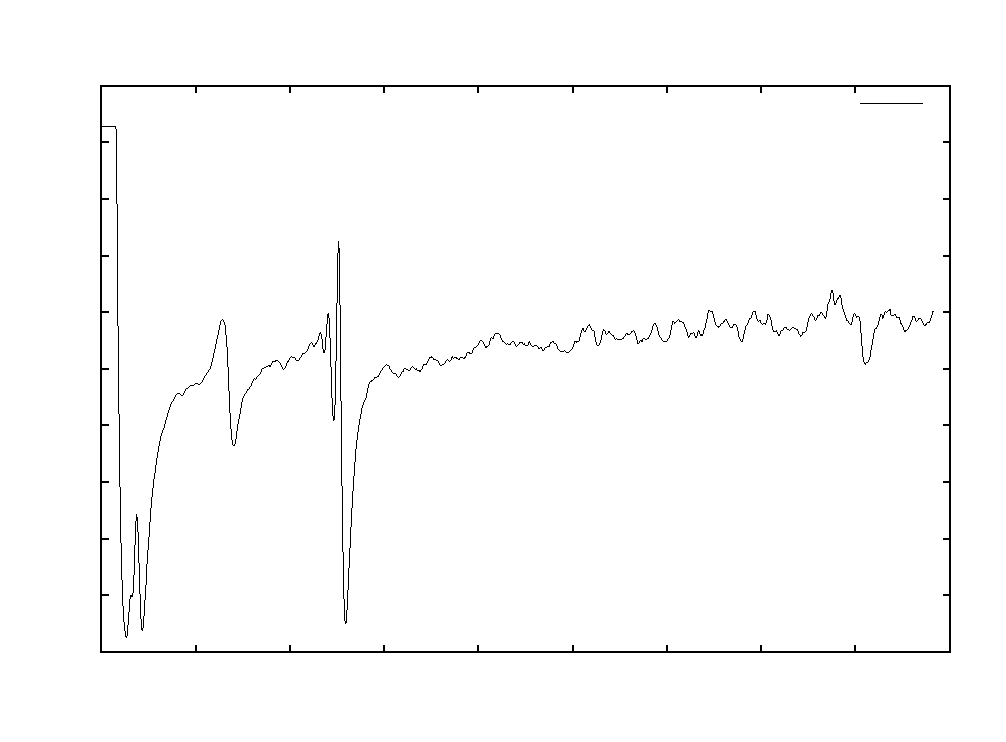
\includegraphics{ma05-03}}%
    \gplfronttext
  \end{picture}%
\endgroup

			\caption{\centering Parameter: Modulationsspannung 5V, AQ 6min, Empfindlichkeit 0.3mV, Zeitkonstante 3s, Phase 12^\circ}
		\end{figure}

		\begin{description}
			\item[Kohlenstoff (C):] $2.23$ bei $280$eV (chemische Verschiebung des Energieniveaus)
			\item[Sauerstoff (O):] $6.76$ bei $518$eV (chemische Verschiebung des Energieniveaus)
			\item[Silizium (Si):] $0.90$ bei $1621$eV
			\item[Silizium (Si):] $2.06$ bei $86$eV
		\end{description}

		Es folgt:

		\begin{itemize}
			\item 
				$c(C) = 0.44$
			\item
				$c(O) = 0.47$
			\item
				$c(Si) = 0.09$
		\end{itemize}

		Der Glanz der Probe auf dem fotografierten Bild und das Auftreten von Silizium und Sauerstoff könnten eine Zusammensetzung ähnlich von Glas ($SiO_2$) vermuten lassen.
		Jedoch zeigen die relativen Konzentrationen damit keine Übereinstimmung.
		Grundsätzlich kann die Probe durch Sauer- und Kohlenstoff auch stark verunreinigt sein. 
		Des Weiteren gibt es die Möglichkeit, das im nicht-aufgenommenen Bereich andere Peaks liegen, welche zusätzliche Aussagen über die Stoffzusammensetzung geben würden (maximaler Span: 2000V).
		Es ist uns nicht möglich anhand des gegebenen Spektrums weitere Aussagen über die Oberfläche der Probe zu treffen.

	% subsubsection probe_3 (end)

% subsection qualitative_analyse_der_proben (end)

\subsection{Einfluss des Elektronenstrahls auf die Probe} % (fold)
\label{sub:einfluss_des_elektronenstrahls_auf_die_probe}

	Folgendes Probenstrombild wurde vor der Messung eines Auger-Spektrums über Probe 3 aufgenommen:

	\begin{figure}[H]
		\center
		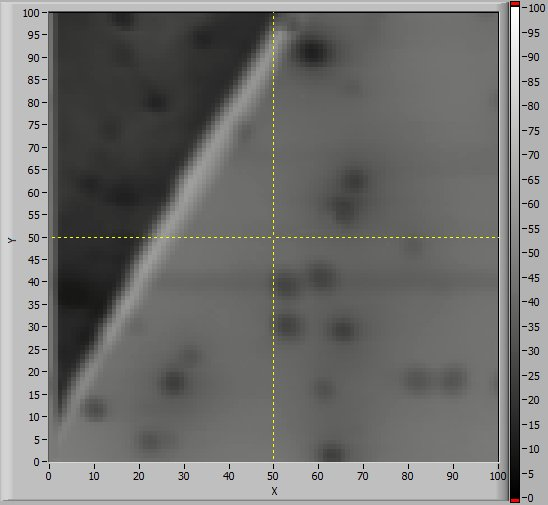
\includegraphics[scale=0.4]{voher.jpg}
		\caption{Probenstrombild der Probe 3 vor der Aufnahme eines Auger-Spektrums}
	\end{figure}

	Durch eine weitere Aufnahme eines Probenstrombilds nach der Messung war nun deutlich, dass der Elektronenstrahl die Oberfläche leicht verändert.

	\begin{figure}[H]
		\center
		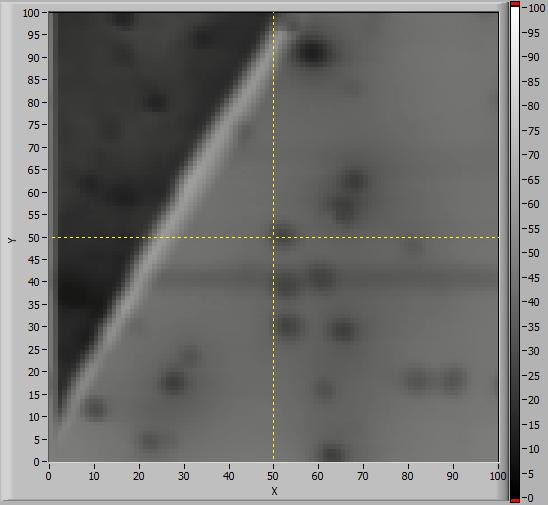
\includegraphics[scale=0.4]{nachher.jpg}
		\caption{Probenstrombild der Probe 3 nach der Aufnahme des Auger-Spektrums}
	\end{figure}

	Die dunkle Verfärbung bedeutet hierbei einen geringeren Probenstrom an der bestrahlten Stelle.
	Es fließen also nicht so viele Elektronen an dieser Stelle ab, wie vorher.
	Sie müssen aus diesem Grund stärker reflektiert werden.
	Dies deutet daraufhin, dass an der untersuchten Stelle das Material glatter geworden ist (bzw. von einer dünnen Verunreinigungsschicht befreit worden ist).

% subsection einfluss_des_elektronenstrahls_auf_die_probe (end)

\newpage

\subsection{Sputtering} % (fold)
\label{sub:sputtering}

	Zum Vergleich bereits oben gezeigtes Silber-Spektrum vor dem Ionenätzen:

	\begin{figure}[H]
		\center
		% GNUPLOT: LaTeX picture with Postscript
\begingroup
  \makeatletter
  \providecommand\color[2][]{%
    \GenericError{(gnuplot) \space\space\space\@spaces}{%
      Package color not loaded in conjunction with
      terminal option `colourtext'%
    }{See the gnuplot documentation for explanation.%
    }{Either use 'blacktext' in gnuplot or load the package
      color.sty in LaTeX.}%
    \renewcommand\color[2][]{}%
  }%
  \providecommand\includegraphics[2][]{%
    \GenericError{(gnuplot) \space\space\space\@spaces}{%
      Package graphicx or graphics not loaded%
    }{See the gnuplot documentation for explanation.%
    }{The gnuplot epslatex terminal needs graphicx.sty or graphics.sty.}%
    \renewcommand\includegraphics[2][]{}%
  }%
  \providecommand\rotatebox[2]{#2}%
  \@ifundefined{ifGPcolor}{%
    \newif\ifGPcolor
    \GPcolorfalse
  }{}%
  \@ifundefined{ifGPblacktext}{%
    \newif\ifGPblacktext
    \GPblacktexttrue
  }{}%
  % define a \g@addto@macro without @ in the name:
  \let\gplgaddtomacro\g@addto@macro
  % define empty templates for all commands taking text:
  \gdef\gplbacktext{}%
  \gdef\gplfronttext{}%
  \makeatother
  \ifGPblacktext
    % no textcolor at all
    \def\colorrgb#1{}%
    \def\colorgray#1{}%
  \else
    % gray or color?
    \ifGPcolor
      \def\colorrgb#1{\color[rgb]{#1}}%
      \def\colorgray#1{\color[gray]{#1}}%
      \expandafter\def\csname LTw\endcsname{\color{white}}%
      \expandafter\def\csname LTb\endcsname{\color{black}}%
      \expandafter\def\csname LTa\endcsname{\color{black}}%
      \expandafter\def\csname LT0\endcsname{\color[rgb]{1,0,0}}%
      \expandafter\def\csname LT1\endcsname{\color[rgb]{0,1,0}}%
      \expandafter\def\csname LT2\endcsname{\color[rgb]{0,0,1}}%
      \expandafter\def\csname LT3\endcsname{\color[rgb]{1,0,1}}%
      \expandafter\def\csname LT4\endcsname{\color[rgb]{0,1,1}}%
      \expandafter\def\csname LT5\endcsname{\color[rgb]{1,1,0}}%
      \expandafter\def\csname LT6\endcsname{\color[rgb]{0,0,0}}%
      \expandafter\def\csname LT7\endcsname{\color[rgb]{1,0.3,0}}%
      \expandafter\def\csname LT8\endcsname{\color[rgb]{0.5,0.5,0.5}}%
    \else
      % gray
      \def\colorrgb#1{\color{black}}%
      \def\colorgray#1{\color[gray]{#1}}%
      \expandafter\def\csname LTw\endcsname{\color{white}}%
      \expandafter\def\csname LTb\endcsname{\color{black}}%
      \expandafter\def\csname LTa\endcsname{\color{black}}%
      \expandafter\def\csname LT0\endcsname{\color{black}}%
      \expandafter\def\csname LT1\endcsname{\color{black}}%
      \expandafter\def\csname LT2\endcsname{\color{black}}%
      \expandafter\def\csname LT3\endcsname{\color{black}}%
      \expandafter\def\csname LT4\endcsname{\color{black}}%
      \expandafter\def\csname LT5\endcsname{\color{black}}%
      \expandafter\def\csname LT6\endcsname{\color{black}}%
      \expandafter\def\csname LT7\endcsname{\color{black}}%
      \expandafter\def\csname LT8\endcsname{\color{black}}%
    \fi
  \fi
  \setlength{\unitlength}{0.0500bp}%
  \begin{picture}(9354.00,5102.00)%
    \gplgaddtomacro\gplbacktext{%
      \csname LTb\endcsname%
      \put(946,704){\makebox(0,0)[r]{\strut{}-2}}%
      \put(946,1171){\makebox(0,0)[r]{\strut{}-1.5}}%
      \put(946,1638){\makebox(0,0)[r]{\strut{}-1}}%
      \put(946,2105){\makebox(0,0)[r]{\strut{}-0.5}}%
      \put(946,2573){\makebox(0,0)[r]{\strut{} 0}}%
      \put(946,3040){\makebox(0,0)[r]{\strut{} 0.5}}%
      \put(946,3507){\makebox(0,0)[r]{\strut{} 1}}%
      \put(946,3974){\makebox(0,0)[r]{\strut{} 1.5}}%
      \put(946,4441){\makebox(0,0)[r]{\strut{} 2}}%
      \put(1078,484){\makebox(0,0){\strut{} 0}}%
      \put(2391,484){\makebox(0,0){\strut{} 100}}%
      \put(3704,484){\makebox(0,0){\strut{} 200}}%
      \put(5018,484){\makebox(0,0){\strut{} 300}}%
      \put(6331,484){\makebox(0,0){\strut{} 400}}%
      \put(7644,484){\makebox(0,0){\strut{} 500}}%
      \put(8957,484){\makebox(0,0){\strut{} 600}}%
      \put(176,2572){\rotatebox{-270}{\makebox(0,0){\strut{}$dN/dE \ [1]$}}}%
      \put(5017,154){\makebox(0,0){\strut{}$E \ [eV]$}}%
      \put(5017,4771){\makebox(0,0){\strut{}Ag-Spektrum}}%
    }%
    \gplgaddtomacro\gplfronttext{%
      \csname LTb\endcsname%
      \put(7970,4268){\makebox(0,0)[r]{\strut{}Messwerte}}%
    }%
    \gplbacktext
    \put(0,0){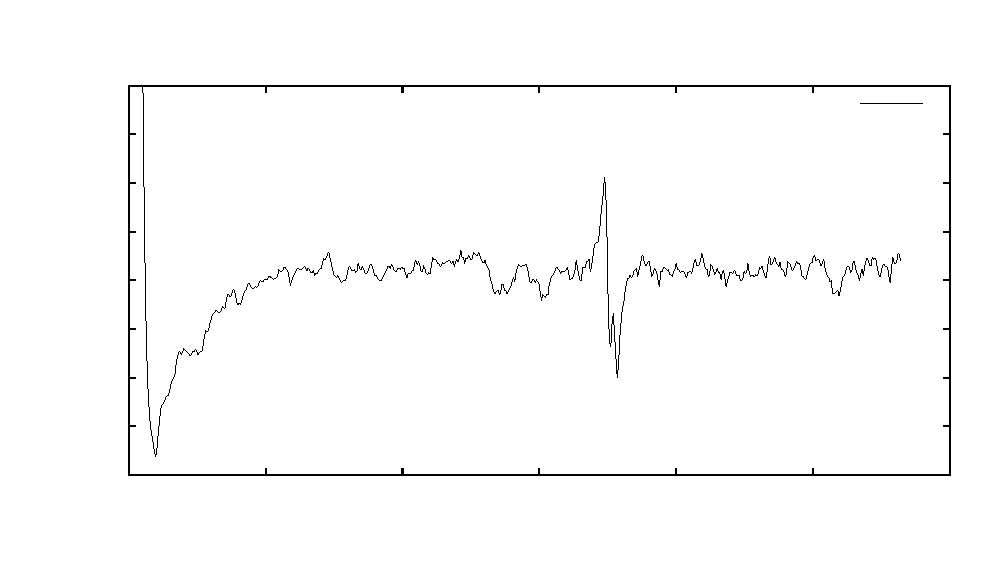
\includegraphics{ma03-16}}%
    \gplfronttext
  \end{picture}%
\endgroup

	\end{figure}

	Nach dem Sputtering:

	\begin{figure}[H]
		\center
		% GNUPLOT: LaTeX picture with Postscript
\begingroup
  \makeatletter
  \providecommand\color[2][]{%
    \GenericError{(gnuplot) \space\space\space\@spaces}{%
      Package color not loaded in conjunction with
      terminal option `colourtext'%
    }{See the gnuplot documentation for explanation.%
    }{Either use 'blacktext' in gnuplot or load the package
      color.sty in LaTeX.}%
    \renewcommand\color[2][]{}%
  }%
  \providecommand\includegraphics[2][]{%
    \GenericError{(gnuplot) \space\space\space\@spaces}{%
      Package graphicx or graphics not loaded%
    }{See the gnuplot documentation for explanation.%
    }{The gnuplot epslatex terminal needs graphicx.sty or graphics.sty.}%
    \renewcommand\includegraphics[2][]{}%
  }%
  \providecommand\rotatebox[2]{#2}%
  \@ifundefined{ifGPcolor}{%
    \newif\ifGPcolor
    \GPcolorfalse
  }{}%
  \@ifundefined{ifGPblacktext}{%
    \newif\ifGPblacktext
    \GPblacktexttrue
  }{}%
  % define a \g@addto@macro without @ in the name:
  \let\gplgaddtomacro\g@addto@macro
  % define empty templates for all commands taking text:
  \gdef\gplbacktext{}%
  \gdef\gplfronttext{}%
  \makeatother
  \ifGPblacktext
    % no textcolor at all
    \def\colorrgb#1{}%
    \def\colorgray#1{}%
  \else
    % gray or color?
    \ifGPcolor
      \def\colorrgb#1{\color[rgb]{#1}}%
      \def\colorgray#1{\color[gray]{#1}}%
      \expandafter\def\csname LTw\endcsname{\color{white}}%
      \expandafter\def\csname LTb\endcsname{\color{black}}%
      \expandafter\def\csname LTa\endcsname{\color{black}}%
      \expandafter\def\csname LT0\endcsname{\color[rgb]{1,0,0}}%
      \expandafter\def\csname LT1\endcsname{\color[rgb]{0,1,0}}%
      \expandafter\def\csname LT2\endcsname{\color[rgb]{0,0,1}}%
      \expandafter\def\csname LT3\endcsname{\color[rgb]{1,0,1}}%
      \expandafter\def\csname LT4\endcsname{\color[rgb]{0,1,1}}%
      \expandafter\def\csname LT5\endcsname{\color[rgb]{1,1,0}}%
      \expandafter\def\csname LT6\endcsname{\color[rgb]{0,0,0}}%
      \expandafter\def\csname LT7\endcsname{\color[rgb]{1,0.3,0}}%
      \expandafter\def\csname LT8\endcsname{\color[rgb]{0.5,0.5,0.5}}%
    \else
      % gray
      \def\colorrgb#1{\color{black}}%
      \def\colorgray#1{\color[gray]{#1}}%
      \expandafter\def\csname LTw\endcsname{\color{white}}%
      \expandafter\def\csname LTb\endcsname{\color{black}}%
      \expandafter\def\csname LTa\endcsname{\color{black}}%
      \expandafter\def\csname LT0\endcsname{\color{black}}%
      \expandafter\def\csname LT1\endcsname{\color{black}}%
      \expandafter\def\csname LT2\endcsname{\color{black}}%
      \expandafter\def\csname LT3\endcsname{\color{black}}%
      \expandafter\def\csname LT4\endcsname{\color{black}}%
      \expandafter\def\csname LT5\endcsname{\color{black}}%
      \expandafter\def\csname LT6\endcsname{\color{black}}%
      \expandafter\def\csname LT7\endcsname{\color{black}}%
      \expandafter\def\csname LT8\endcsname{\color{black}}%
    \fi
  \fi
  \setlength{\unitlength}{0.0500bp}%
  \begin{picture}(9354.00,5102.00)%
    \gplgaddtomacro\gplbacktext{%
      \csname LTb\endcsname%
      \put(682,704){\makebox(0,0)[r]{\strut{}-4}}%
      \put(682,1078){\makebox(0,0)[r]{\strut{}-3}}%
      \put(682,1451){\makebox(0,0)[r]{\strut{}-2}}%
      \put(682,1825){\makebox(0,0)[r]{\strut{}-1}}%
      \put(682,2199){\makebox(0,0)[r]{\strut{} 0}}%
      \put(682,2573){\makebox(0,0)[r]{\strut{} 1}}%
      \put(682,2946){\makebox(0,0)[r]{\strut{} 2}}%
      \put(682,3320){\makebox(0,0)[r]{\strut{} 3}}%
      \put(682,3694){\makebox(0,0)[r]{\strut{} 4}}%
      \put(682,4067){\makebox(0,0)[r]{\strut{} 5}}%
      \put(682,4441){\makebox(0,0)[r]{\strut{} 6}}%
      \put(814,484){\makebox(0,0){\strut{} 0}}%
      \put(2171,484){\makebox(0,0){\strut{} 100}}%
      \put(3528,484){\makebox(0,0){\strut{} 200}}%
      \put(4886,484){\makebox(0,0){\strut{} 300}}%
      \put(6243,484){\makebox(0,0){\strut{} 400}}%
      \put(7600,484){\makebox(0,0){\strut{} 500}}%
      \put(8957,484){\makebox(0,0){\strut{} 600}}%
      \put(176,2572){\rotatebox{-270}{\makebox(0,0){\strut{}$dN/dE \ [1]$}}}%
      \put(4885,154){\makebox(0,0){\strut{}$E \ [eV]$}}%
      \put(4885,4771){\makebox(0,0){\strut{}Silber-Spektrum nach Sputtering}}%
    }%
    \gplgaddtomacro\gplfronttext{%
      \csname LTb\endcsname%
      \put(7970,4268){\makebox(0,0)[r]{\strut{}Messwerte}}%
    }%
    \gplbacktext
    \put(0,0){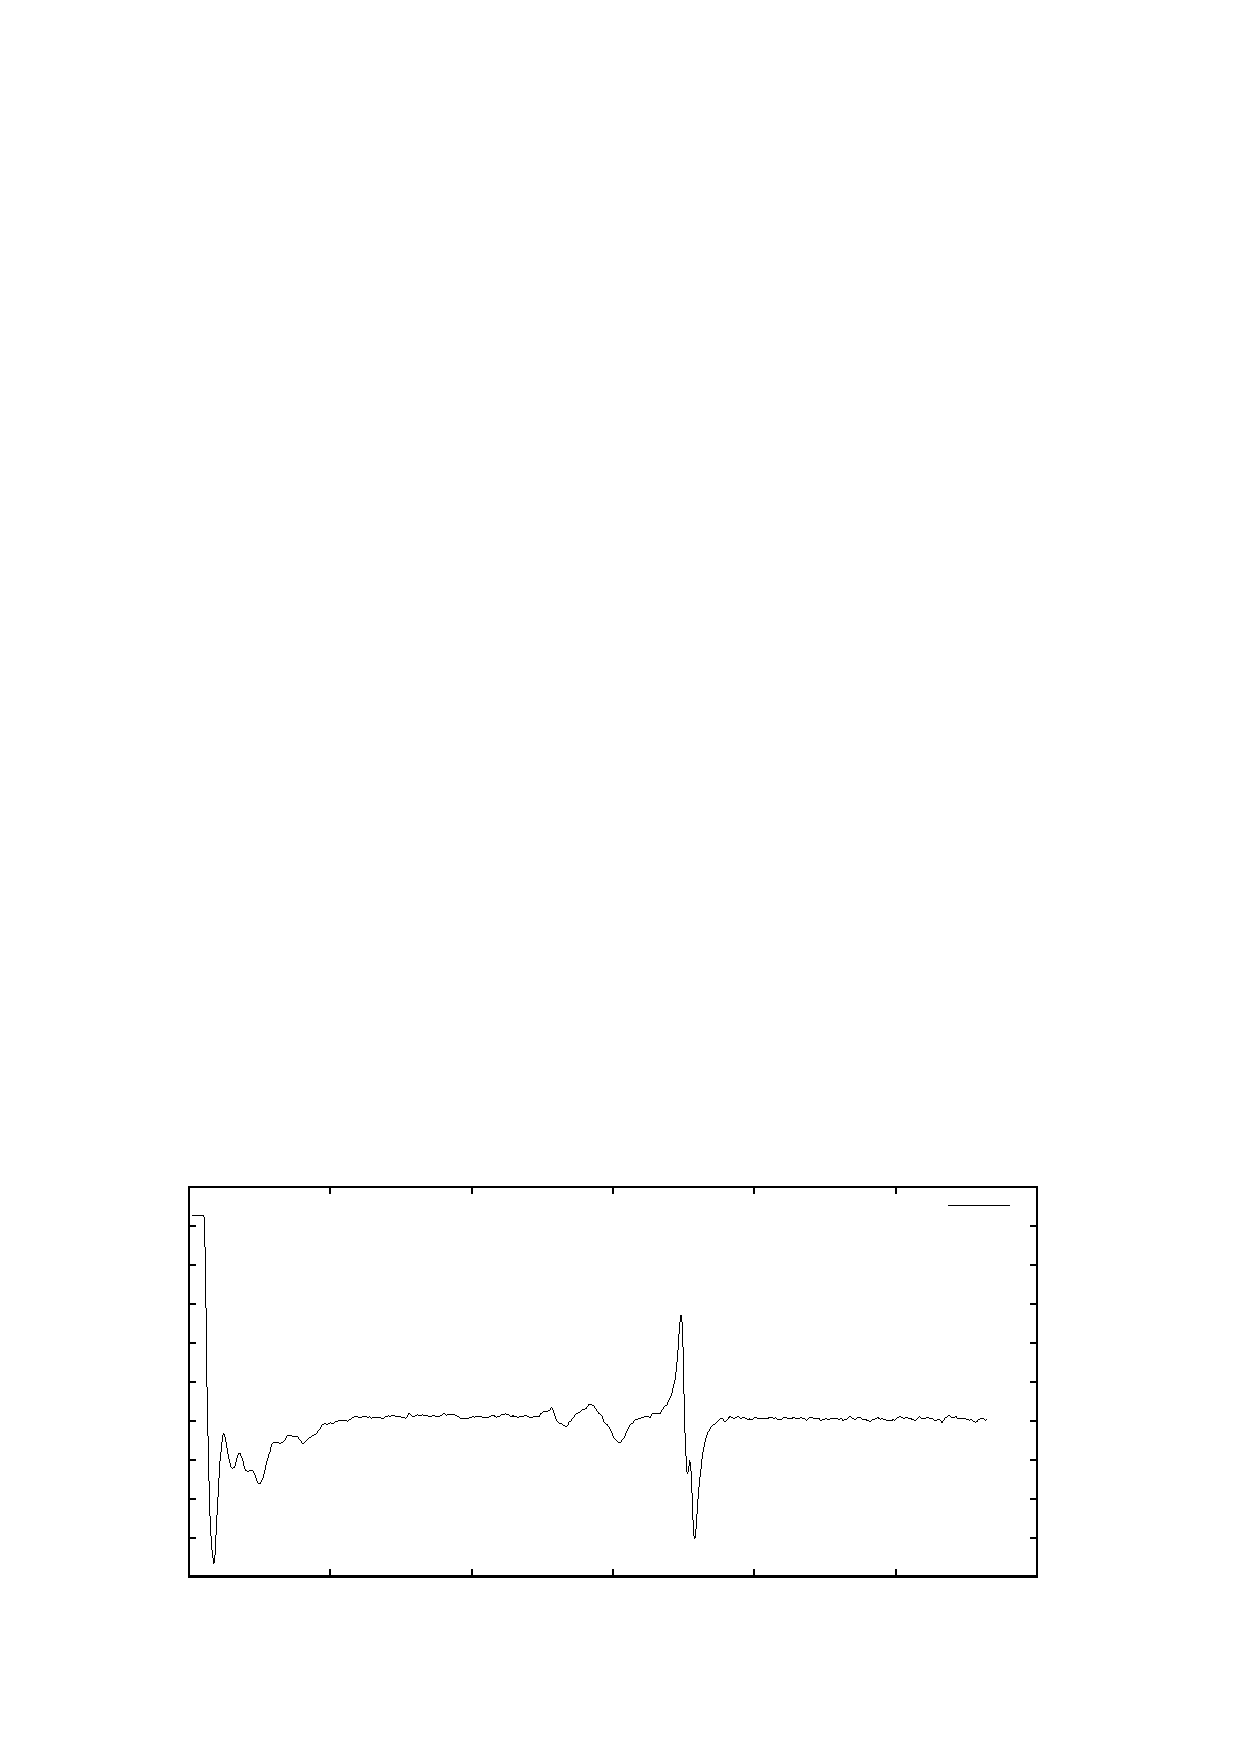
\includegraphics{agg}}%
    \gplfronttext
  \end{picture}%
\endgroup

		\caption{\centering Parameter: Modulationsspannung 2V, AQ 4min, Empfindlichkeit 1mV, Zeitkonstante 1s, Phase 12^\circ }
	\end{figure}

	Die stark geglättete Kurve zeigt, dass durch das Ionenätzen viele Verunreinigungen und Spurenelemente von der Oberfläche entfernt werden konnten, 
	sodass außer den charakteristischen Silberpeaks kaum noch andere Signale auftreten.


% subsection sputtering (end)